%definira klasu dokumenta 
\documentclass[12pt]{report} 

%prostor izmedu naredbi \documentclass i \begin{document} se zove uvod. U njemu se nalaze naredbe koje se odnose na cijeli dokument

%osnovni LaTex ne može riješiti sve probleme, pa se koriste različiti paketi koji olakšavaju izradu željenog dokumenta
\usepackage[croatian]{babel} 
\usepackage{amssymb}
\usepackage{amsmath}
\usepackage{txfonts}
\usepackage{mathdots}
\usepackage{titlesec}
\usepackage{array}
\usepackage{lastpage}
\usepackage{etoolbox}
\usepackage{longtable, tabu}
\usepackage{color, colortbl}
\usepackage{adjustbox}
\usepackage{geometry}
\usepackage[classicReIm]{kpfonts}
\usepackage{hyperref}
\usepackage{fancyhdr}

\usepackage{float}
\usepackage{setspace}
\restylefloat{table}


\patchcmd{\chapter}{\thispagestyle{plain}}{\thispagestyle{fancy}}{}{} %redefiniranje stila stranice u paketu fancyhdr

%oblik naslova poglavlja
\titleformat{\chapter}{\normalfont\huge\bfseries}{\thechapter.}{20pt}{\Huge}
\titlespacing{\chapter}{0pt}{0pt}{40pt}


\linespread{1.3} %razmak između redaka

\geometry{a4paper, left=1in, top=1in,}  %oblik stranice

\hypersetup{ colorlinks, citecolor=black, filecolor=black, linkcolor=black,	urlcolor=black }   %izgled poveznice


%prored smanjen između redaka u nabrajanjima i popisima
\newenvironment{packed_enum}{
	\begin{enumerate}
		\setlength{\itemsep}{0pt}
		\setlength{\parskip}{0pt}
		\setlength{\parsep}{0pt}
	}{\end{enumerate}}

\newenvironment{packed_item}{
	\begin{itemize}
		\setlength{\itemsep}{0pt}
		\setlength{\parskip}{0pt}
		\setlength{\parsep}{0pt}
	}{\end{itemize}}


%boja za privatni i udaljeni kljuc u tablicama
\definecolor{LightBlue}{rgb}{0.9,0.9,1}
\definecolor{LightGreen}{rgb}{0.9,1,0.9}


%podesavanje zaglavlja i podnožja

\pagestyle{fancy}
\lhead{Programsko inženjerstvo}
\rhead{GeoFighter}
\lfoot{Ferllowship}
\cfoot{stranica \thepage/\pageref{LastPage}}
\rfoot{\today}
\renewcommand{\headrulewidth}{0.2pt}
\renewcommand{\footrulewidth}{0.2pt}


\begin{document} 
	
	
	
	\begin{titlepage}
		\begin{center}
			\vspace*{\stretch{1.0}} %u kombinaciji s ostalim \vspace naredbama definira razmak između redaka teksta
			\LARGE Programsko inženjerstvo\\
			\large Ak. god. 2020./2021.\\
			
			\vspace*{\stretch{3.0}}
			
			\huge GeoFighter\\
			\Large Dokumentacija, Rev. \textit{$<$1 ili 2$>$}\\
			
			\vspace*{\stretch{12.0}}
			\normalsize
			Grupa: \textit{Ferllowship}\\
			Voditelj: \textit{Matija Frandolić}\\
			
			
			\vspace*{\stretch{1.0}}
			Datum predaje: \textit{$<$dan$>$. $<$mjesec$>$. $<$godina$>$.}\\
	
			\vspace*{\stretch{4.0}}
			
			Nastavnik: \textit{Hrvoje Nuić}\\
		
		\end{center}

	
	\end{titlepage}

	
	\tableofcontents

	\chapter{Dnevnik promjena dokumentacije}
						
		\begin{longtabu} to \textwidth {|X[2, l]|X[13, l]|X[3, l]|X[3, l]|}
			\hline \multicolumn{1}{|l|}{\textbf{Rev.}} & \multicolumn{1}{l|}{\textbf{Opis promjene/dodatka}} & \multicolumn{1}{l|}{\textbf{Autori}} & \multicolumn{1}{l|}{\textbf{Datum}} \\[3pt] \hline
			\endfirsthead
			
			\hline \multicolumn{1}{|l|}{\textbf{Rev.}} & \multicolumn{1}{l|}{\textbf{Opis promjene/dodatka}} & \multicolumn{1}{l|}{\textbf{Autori}} & \multicolumn{1}{l|}{\textbf{Datum}} \\[3pt] \hline
			\endhead
			
			\hline 
			\endlastfoot
			
			0.1 & Napravljen predložak & Frandolić & 07.10.2020. \\[3pt] \hline 
			0.2	& Dodani uvod i razrada u opis projektnog zadatka \smallskip & Kopić & 17.10.2020. \\[3pt] \hline 
			0.3 & Dodan ostatak opisa projektnoga zadatka (potencijalne koristi, korisnici i moguće nadogradnje) \smallskip & Kopić & 20.10.2020. \\[3pt] \hline 
			0.4 & Dodani funkcionali zahtjevi & Bašić & 20.10.2020. \\[3pt] \hline 
			0.5.1 & Dodan prvi dio opisa obrazaca uporabe & Krivačić & 20.10.2020. \\[3pt] \hline
			0.5.2 & Dodan drugi dio opisa obrazaca uporabe & Bašić Krivačić \smallskip & 21.10.2020. \\[3pt] \hline
			0.6 & Dodani dijagrami obrazaca uporabe & Krivačić & 25.10.2020. \\[3pt] \hline
			0.7 & Dodani sekvencijski dijagrami & Bašić Krivačić \smallskip & 28.10.2020. \\[3pt] \hline
			0.8 & Dodana postojeća slična rješenja u Opis projektnoga zadatka \smallskip & Kopić & 29.10.2020. \\[3pt] \hline 
			0.9.1 & Dodan opis i dijagrami baze podataka & Petrović Brečić \smallskip & 05.11.2020. \\[3pt] \hline
			0.9.2 & Izmjene u opisu baze podataka & Petrović Brečić \smallskip & 12.11.2020. \\[3pt] \hline 
			0.10.1 & Dodani opis i prvi dijagrami razreda & Brečić Petrović \smallskip & 12.11.2020. \\[3pt] \hline 
			0.10.2 & Izmjenjen opis arhitekture sustava i dovršeni dijagrami razreda & Brečić Krivačić Kopić \smallskip & 13.11.2020. \\[3pt] \hline 
			
			\textbf{1.0} & Pregledano prije predaje za 1. ciklus & Frandolić & 13.11.2020. \\[3pt] \hline 
			
			1.1 & Dodan predložak za drugu reviziju & Frandolić & 30.12.2020. \\[3pt] \hline 
			
			1.2 & Dodan dijagram komponenti & Kopić & 13.1.2021. \\[3pt] \hline 
			1.3 & Dodan dijagram aktivnosti & Petrović & 14.1.2021. \\[3pt] \hline
%			\textbf{2.0} & Konačna verzija & Ivošević & 28.09.2013. \\[3pt] \hline 
			
		\end{longtabu}

	\chapter{Opis projektnog zadatka}
		
		\textbf{\textit{\large 2.1 Uvod}}\\
		
		{Kroz ovaj je projekt potrebno razviti programsku potporu za igru  \emph{GeoFighter}. \emph{GeoFighter} je web-aplikacija kojom se u obliku karata određenih jačina evidentiraju stvarne lokacije koje su korisnici (č. igrači) posjetili. Skupljenim se kartama tada geografski bliski igrači mogu međusobno boriti. Pobjednik borbe dobiva određeni broj bodova koji se oduzimaju gubitniku te se promjenom bodova mijenja i globalni rang igrača. Cilj igrača je posjetiti što veći broj mjesta, skupiti što više karata i postići što bolji rang. } \\
		
		
		\textbf{\textit{\large 2.2 Razrada }}\\ 
		
		\textbf{\textit{2.2.1 Registracija i prijava }}\\
		
		{Prije korištenja same aplikacije, ukoliko je korisnik novi igrač, dužan je najprije registrirati se. Za registraciju potrebni su:}
	
		\begin{packed_item}
			\item {korisničko ime,}
			\item {fotografija,}
			\item {lozinka,}
			\item {e-mail adresa.}
		\end{packed_item}
		
		{Validacijom podataka utvrđuje se ispravnost unosa podataka te se provjerava postoji li već korisnik s istim korisničkim imenom ili e-mail adresom. Kada registracije bude gotova, korisniku se na navedenu adresu šalje poveznica putem koje potvrđuje svoj račun. Tek nakon što je račun potvrđen, omogućuje se ulazak u sâm igrački sustav.}
		{Ako je igrač već prethodno registriran, on u sustav ulazi upisujući korisničko ime ili e-mail adresu, i lozinku.}\\ \\ \\
		
		\textbf{\textit{2.2.2 Korištenje sustava}}\\
		
		\textbf{\textit{\small2.2.2.1 Početni zaslon i mogućnosti}}\\
		
		
		{Pri ulasku u sustav korisniku se na karti prikazuje njegova lokacija zajedno s obližnjim lokacijama. Pritiskom na određenu lokaciju otvara se prozor s atributima poput naziva lokacije, opisa, fotografije, kategorije i jačina karte te lokacije. Kategorije lokacija uključuju naseljena mjesta, vrhove planina i gora, umjetničke instalacije... Na zaslonu se nalazi simbol za padajući izbornik. Pritiskom na taj simbol, izbornik se otvara na vrhu ili sa strane, ovisno o veličini ekrana, te prikazuje simbole koji označavaju:  }
		
			\begin{packed_item}
			\item {\textbf{Profil korisnika }- otvara novi prozor u kojem se prikazuju podatci o korisniku(korisničko ime, fotografija, lozinka, e-mail adresa). Za fotografiju i korisničko ime sa strane nudi se mogućnost uređivanja.}\\
			\item {\textbf{Kolekciju korisnikovih karata} - otvara novi prozor unutar kojega su prikazane karte koje je korisnik skupio. Karte je zatim moguće poredati prema kategorijama ili prema jačini.}\\
			\item {\textbf{Globalnu rang ljestvicu} - otvara novi prozor koji prikazuje redne brojeve igrača, njihova korisnička imena i brojeve bodova poredane silazno.}\\
			\item {\textbf{Pomoć korisniku} - otvara prozor putem kojega se korisnici prijavljuju za ulogu kartografa. Osim toga, ovaj prozor nudi mogućnosti prijave da određena lokacija postane nova karta te kontaktiranja administratora ukoliko korisnik ima primjedbi ili prijedloga. }
			\end{packed_item}
		
		{Izbornik se zatvara ponovnim klikom na njegov simbol te se vraća početni zaslon. Igrač zatim svoje stvarno kretanje prati na karti te pokušava obići što više stvarnih lokacija. Kada igrač stigne na neku lokaciju koja je označena kao karta, pojavljuje se poruka koja javlja da korisnik ima novu lokaciju u kolekciji karata te prikazuje atribute te lokacije.}\newpage
		
		\textbf{\textit{\small2.2.2.2 Borba}}\\
		
		Ukoliko korisnik ugleda na karti u krugu od 50 km drugoga igrača s kojim se želi boriti, pritiskom na drugog igrača pojavljuje se prozor u kojemu onda potvrđuje slanje pozivnice za borbu ili odustaje od izazova. S druge strane, drugome se  igraču prikazuje iskočni prozor s ponudom za borbu i podatcima o protivniku kao što su korisničko ime, broj bodova i trenutačni rang. Tada drugi igrač može prihvatiti ili odbiti borbu. \\
			 
		Ako je borba prihvaćena, svaki od igrača naizmjence bira po jednu kategoriju karata u kojoj će se boriti po rundama. Borba se odvija u tri runde, stoga igrač koji inicira borbu može izabrati dvije kategorije, a izazvani igrač samo jednu. Borbu prvi započinje igrač s manjim globalnim rangom. On odabire jednu od svojih karata iz prethodno odabrane kategorije i baca ju. Drugi igrač zatim iz svojega špila također odabire kartu iz te kategorije i baca ju. Jača karta pobjeđuje te sljedeću rundu otvara pobjednik prethodne runde. Ako igra bude odlučena nakon prve dvije runde, do treće ni ne dolazi. Tada pobjednik dobiva broj bodova koji odgovara broju bodova najjače karte, dok se isti taj broj bodova oduzima gubitniku. Karte korištene u borbi zatim slabe za broj bodova koji imaju podijeljen sa 100. Prozor s borbom se zatvara kod oba igrača te im se prikazuje ažuriranje njihovih osobnih bodova i bodova karata iz kojega se zatim vraća na početni zaslon. \\
		
		
		\textbf{\textit{\small2.2.2.3 Bodovanje karata}}\\
		
		{Svaka karta ima broj bodova koji mu daje kategorija kojoj pripada. Što je kategorija rjeđa i teža za posjetiti (npr. vrh planine naspram nekoga grada) to donosi više bodova. Svaka karta osim toga ima i početnih 100 bodova koji se onda smanjuju za 0.25 boda za svaku posjetu toj lokaciji. Minimalni broj tih bodova 0. Ukupan broj bodova neke karte je zbroj tih dvaju vrijednosti.\\ }
		
		
		\begin{tabular}{ll}
			\textbf{Naziv kategorije} & \textbf{Broj bodova} \\
			Grad                      & 25                   \\
			Naselje                   & 30                   \\
			Umjetnička instalacija    & 35                   \\
			Vrh planine               & 40                   \\
				&                     
		\end{tabular}
	
		
		\textbf{\textit{2.2.3 Održavanje sustava}}\\
		 
		\textbf{\textit{\small2.2.3.1 Administratori}}\\
		
		{Administratori imaju sve ovlasti kao i ostali registrirani korisnici uz još neke dodatne. Oni imaju pristup bazi podataka i mogućnost uređivanja profila korisnika. Administratori također pregledavaju prijave za kartografe i odobravaju ih ili odbijaju. Osim toga, ukoliko korisnici pošalju pitanja unutar prozora za pomoć, oni na njih odgovaraju.} \\
		
		\textbf{\textit{\small2.2.3.2 Kartografi}}\\
		
		{Ako korisniku administrator odobri status kartografa, prije nego što počne koristiti svoje kartografske ovlasti, on mora u svoje korisničke podatke dodati IBAN računa za uplatu i fotografiju osobne iskaznice. Kartografi su osobe zadužene za nadopunjavanje baze podataka s lokacijama koje su igrači prijavili za moguće proširenje. Njima se u padajućem izborniku pojavljuje posebni gumb pomoću kojega se otvara prozor s prijedlozima za nove lokacije. Osim toga, prijedlozi im se prikazuju na karti, a oni ih mogu odbiti, potvrditi, urediti ili označiti da je potrebna potvrda s terena. Kartograf za one prijave za koje je potrebno potvrđivanje s terena može označiti da će ih osobno doći provjeriti, a sustav mu preko vanjskog servisa OSRM dohvaća najbliži put do lokacije.} \\
		
		\textbf{\textit{\large 2.3 Potencijalne koristi}}\\
		
		{Geofighter potiče igrače na istraživanje onih manje poznatih ili čak neotkrivenih lokacija oko njih. Osim toga, korisnika se obogaćuje novim znanjima pomoću informacija o lokacijama na kartama i motivira na otkrivanje novih kultura što dovodi do razvijanja međuljudskih odnosa.} \newpage
		
		\textbf{\textit{\large 2.4 Korisničke skupine}}\\
		
		{Ova je aplikacija prije svega namijenjena ljudima natjecateljskoga duha koji uz to vole i putovati ili jednostavno onima koji žele naučiti nove informacije o već poznatim lokacijama kroz igru. Igrači bi trebali biti boljeg fizičkog stanja kako bi došli do teže dostupnih lokacija te biti punoljetne kako bi se mogle kretati bez većih zakonskih ograničenja. Skupine igrača koje najviše odgovaraju opisu su osobe od oko 20 do oko 50 godina, neovisno kojega spola.}\\
		
		\textbf{\textit{\large 2.5 Moguće nadogradnje}}\\
		
		{Kao moguće nadogradnje naveli bismo:
		\begin{packed_item}
			\item {\textbf{Prozor za razgovor između igrača} - igrači unutar 50 km imali bi mogućnosti jedni drugima poslati poruke tijekom istraživanja karte i tijekom borbe.}\\
			\item {\textbf{Organizacija turnira} - unutar igre bi se organizirali turniri nakon kojih bi pobjednici dobivali određeni broj bodova ili, u daljoj budućnosti i u potencijalnoj suradnji sa zainteresiranim turističkim agencijama koje bi zauzvrat dobivale reklame, putovanja na neke od lokacija na kartama.}\\
			\item {\textbf{Proširenje udaljenosti za borbu} - udaljenost od 50 km unutar koje se igrači mogu boriti bi se potencijalno mogla povećati.} \\
	\end{packed_item} } 
		
		\textbf{\textit{\large 2.6 Postojeća slična rješenja}} \\
		
		{GeoFighter bi se mogao definirati kao hibrid između igara proširene stvarnosti u kojima korisnici putuju stvarnim lokacijama kako bi pristupili lokacijama, artifaktima i sl. unutar igre poput: Harry Potter: Wizards Unite, Pokemon GO, Ingress, The Walking Dead: Our World... i igara u kojima igrači skupljaju karte kao što su: Faeria, Hearthstone, Magic: The Gathering Arena... Kao sustave s najsličnijim specifikacijama treba izdvojiti Pokemon GO - igru u kojoj igrači na stvarnim lokacijama skupljaju Pokemone raznih rijetkosti, posjećuju tzv. Pokemon dvorane u kojima se mogu boriti s drugim stvarnim igračima te skupljati bodove i tako dalje napredovati. Pokemon GO kao framework aplikacije koristi Libgdx i programske jezike Javu, C++ i C\#. Osim Pokemon GO-a trebalo bi izdvojiti i Hearthstone - igru u kojoj igrači skupljaju karte iz različitih kategorija u dekove kako bi se zatim njima borili s drugim igračima. Hearthstone je rađen pomoću Unity-ja, pokretača igara za više platformi, u  C\#.  }
		\eject
	
	\chapter{Specifikacija programske potpore}
		
	\section{Funkcionalni zahtjevi}			
			
			\noindent \textbf{Dionici:}
			
			\begin{packed_enum}
				
				\item Igrači
				\item Kartografi
				\item Administrator			
				\item Razvojni tim
				
			\end{packed_enum}
			
			\noindent \textbf{Aktori i njihovi funkcionalni zahtjevi:}
			
			
			\begin{packed_enum}
				\item  \underbar{Neregistrirani/neprijavljeni korisnik (inicijator) može:}
				
				\begin{packed_enum}
					
					\item obaviti registraciju:
						\begin{packed_enum}
							\item kao igrač  unosom korisničkog imena, fotografije, e-mail adrese i lozinke
							\item kao kartograf unosom korisničkog imena, fotografije, e-mail adrese, lozinke, IBAN-a te fotografije osobne iskaznice
						\end{packed_enum}
					\item ukoliko je korisnik već registriran u sustavu, mora se prijaviti koristeći korisničko ime ili e-mail adresu i lozinku
				\end{packed_enum}
			
				\item  \underbar{Igrač (inicijator) može:}
					
					\begin{packed_enum}
					
						\item pregledavati i mijenjati svoje korisničke podatke
						\item izbrisati svoj korisnički račun
						\item vidjeti kartu na kojoj su označene lokacije na kojima se mogu skupiti karte te njegova lokacija
						\item vidjeti informacije o lokacijama (naziv, opis, fotografiju, kategoriju i jačinu karte te lokacije)
						\item vidjeti kolekciju svojih karata
						\item vidjeti popis ostalih aktivnih igrača koji se nalaze u krugu od 50km i s njima ući u borbu
						\item prijaviti novu lokaciju
						\item vidjeti globalnu statistiku odigranih borbi i sakupljenih lokacija
						\item vidjeti poredak svih igrača
						\item vidjeti profil drugog igrača (njegove karte, rang na globalnoj ljestvici i statistike vezane uz zadnjih 10 borbi s drugim igračima)
					
					\end{packed_enum}
				
				\item  \underbar{Kartograf (inicijator) može:}
				
				\begin{packed_enum}
					
					\item vidjeti kartu sa:
					\begin{packed_enum}
						
						\item prijavljenim lokacijama za unos u bazu podataka
						\item prikazanim najkraćim putem do lokacije koju treba provjeriti na terenu
						\item već unesenim lokacijama u bazi podataka
					
					\end{packed_enum}
					
					\item odbiti, potvrditi, urediti ili označiti da je potrebna potvrda s terena za prijavljenu lokaciju
					\item dodavati lokacije u bazu podataka
					\item vidjeti i izmjeniti svoje osobne podatke
					
				\end{packed_enum}
			
				\item  \underbar{Administrator (inicijator) može:}
				
				\begin{packed_enum}
					
					\item vidjeti i uređivati popis svih korisnika i njihovih osobnih podataka
					\item dodjeliti igračima privremeno isključenje iz igre
					\item vidjeti i uređivati postojeće lokacije
					\item vidjeti globalnu statistiku odigranih borbi i sakupljenih lokacija
					\item vidjeti poredak svih igrača
					
				\end{packed_enum}
			
				\item  \underbar{Baza podataka (sudionik):}
				
				\begin{packed_enum}
					
					\item pohranjuje sve podatke o korisnicima i njihovim ovlastima
					\item  pohranjuje sve podatke o kartama i lokacijama
					\item  pohranjuje sve podatke o borbama i rang listama igrača
					
				\end{packed_enum}
			\end{packed_enum}
			
			\eject 
			
			
				
			\subsection{Obrasci uporabe}
		
				\subsubsection{Opis obrazaca uporabe}
				
					\noindent \underbar{\textbf{UC1 - Početni zaslon za neprijavljenog korisnika}}
					\begin{packed_item}
						
						\item \textbf{Glavni sudionik: }Korisnik
						\item  \textbf{Cilj:} Prikaz početnog zaslona za neprijavljenog korisnika
						\item  \textbf{Sudionici:} Baza podataka
						\item  \textbf{Preduvjet:} -
						\item  \textbf{Opis osnovnog tijeka:}
						
						\item[] \begin{packed_enum}
							
							\item Korisnik pristupa aplikaciji
							\item Otvara se početni zaslon za neprijavljenog korisnika
						\end{packed_enum}
					\end{packed_item}
					
					
					\noindent \underbar{\textbf{UC2 -Registracija igrača}}
					\begin{packed_item}
	
						\item \textbf{Glavni sudionik: }Korisnik
						\item  \textbf{Cilj:} Stvoriti korisnički račun za pristup sustavu
						\item  \textbf{Sudionici:} Baza podataka
						\item  \textbf{Preduvjet:} -
						\item  \textbf{Opis osnovnog tijeka:}
						
						\item[] \begin{packed_enum}
	
							\item Korisnik odabire opciju za registraciju igrača
							\item Korisnik unosi potrebne korisničke podatke(korisničko ime, e-mail, lozinka)
							\item Korisnik prima obavijest o uspješnoj registraciji
							\item Nakon registracije korisnik automatski prijavljen u sustav
						\end{packed_enum}
						
						\item  \textbf{Opis mogućih odstupanja:}
						
						\item[] \begin{packed_item}
	
							\item[2.a] Odabir već zauzetog korisničkog imena i/ili e-maila ili pružanje neispravnog e-maila
							\item[] \begin{packed_enum}
								
								\item Sustav obavještava korisnika o neuspjelom upisu i vraća ga na stranicu za registraciju 
								\item Korisnik mijenja potrebne podatke te završava unos ili odustaje od registracije
								
							\end{packed_enum}
							\item[2.b] Odabir "slabe" lozinke(za "jaku" lozinku obavezno barem 8 znakova, 1 veliko slovo, 1 broj)
							\item[] \begin{packed_enum}
								\item Sustav obavještava korisnika da je lozinka "slaba" i vraća ga na stranicu za registraciju
								\item Korisnik odabire "jaču" lozinku te završava unos ili odustaje od registracije 
								
							\end{packed_enum}
								
						\end{packed_item}
					\end{packed_item}
				
					\noindent \underbar{\textbf{UC3 -Prijava u sustav}}
					\begin{packed_item}
						
						\item \textbf{Glavni sudionik: }Igrač
						\item  \textbf{Cilj:} Dobiti pristup korisničkom sučelju
						\item  \textbf{Sudionici:} Baza podataka
						\item  \textbf{Preduvjet:} Registracija
						\item  \textbf{Opis osnovnog tijeka:}
						
						\item[] \begin{packed_enum}
							
							\item Unos korisničkog imena ili e-maila i lozinke
							\item Potvrda o ispravnosti unesenih podataka
							\item Pristup korisničkim funkcijama
						\end{packed_enum}
						
						\item  \textbf{Opis mogućih odstupanja:}
						
						\item[] \begin{packed_item}
							
							\item[2.a] Unos neispravnog korisničkog imena, e-maila ili lozinke
							\item[] \begin{packed_enum}
								
								\item Sustav obavještava korisnika o neispravnom upisu i vraća ga na stranicu za prijavu
								
							\end{packed_enum}
							
						\end{packed_item}
					\end{packed_item}
					
					\noindent \underbar{\textbf{UC4 - Prijava za kartografa}}
					\begin{packed_item}
						
						\item \textbf{Glavni sudionik: }Igrač
						\item  \textbf{Cilj:} Proširenje ovlasti igrača
						\item  \textbf{Sudionici:} Baza podataka
						\item  \textbf{Preduvjet:} -
						\item  \textbf{Opis osnovnog tijeka:}
						
						\item[] \begin{packed_enum}
							
							\item Korisnik odabire opciju prijava za kartografa
							\item Korisnik unosi potrebne korisničke podatke(IBAN računa za uplatu i fotografiju osobne iskaznice)
							\item Korisnik prima obavijest o uspješnoj prijavi za kartografa te čeka odobrenje administratora
						\end{packed_enum}
						
						\item  \textbf{Opis mogućih odstupanja:}
						
						\item[] \begin{packed_item}
							
							\item[2.a] Neispravan unos IBAN-a
							\item[] \begin{packed_enum}
								
								\item Sustav obavještava korisnika o pogrešnom unosu
								\item Korisnik mijenja potrebne podatke te završava unos ili odustaje od prijave
								
							\end{packed_enum}
							
						\end{packed_item}
					\end{packed_item}
					
					\noindent \underbar{\textbf{UC5 - Pregled lokacija na karti}}
					\begin{packed_item}
						
						\item \textbf{Glavni sudionik: }Igrač
						\item  \textbf{Cilj:} Pregled lokacija koje igrač može posjetiti
						\item  \textbf{Sudionici:} Baza podataka
						\item  \textbf{Preduvjet:} Igrač je prijavljen
						\item  \textbf{Opis osnovnog tijeka:}
						
						\item[] \begin{packed_enum}
							
							\item Korisnik odabire opciju pregled lokacija na karti
							\item Otvara karta s lokacijama
						\end{packed_enum}
					\end{packed_item}
					
					\noindent \underbar{\textbf{UC6 -Pregled informacija o lokaciji}}
					\begin{packed_item}
						
						\item \textbf{Glavni sudionik: }Igrač
						\item  \textbf{Cilj:} Pregled informacija o lokaciji
						\item  \textbf{Sudionici:} Baza podataka
						\item  \textbf{Preduvjet:} Igrač je prijavljen
						\item  \textbf{Opis osnovnog tijeka:}
						
						\item[] \begin{packed_enum}
							
							\item Korisnik odabire opciju "Informacija o lokaciji"
							\item Aplikacija prikazuje informacije o lokaciji
						\end{packed_enum}
					\end{packed_item}
					
					
					\noindent \underbar{\textbf{UC7 -Pregled osobnih podataka igrača}}
					\begin{packed_item}
					
					\item \textbf{Glavni sudionik: }Igrač
					\item  \textbf{Cilj:} Pregledati osobne podatke
					\item  \textbf{Sudionici:} Baza podataka
					\item  \textbf{Preduvjet:} Igrač je prijavljen
					\item  \textbf{Opis osnovnog tijeka:}
					
					\item[] \begin{packed_enum}
						
						\item Korisnik odabire opciju "Osobni podatci"
						\item Aplikacija prikazuje osobne podatke korisnika
					\end{packed_enum}
					\end{packed_item}
			
					\noindent \underbar{\textbf{UC8 -Promjena osobnih podataka igrača}}
					\begin{packed_item}
					
					\item \textbf{Glavni sudionik: }Igrač
					\item  \textbf{Cilj:} Promjeniti osobne podatke
					\item  \textbf{Sudionici:} Baza podataka
					\item  \textbf{Preduvjet:} Igrač je prijavljen
					\item  \textbf{Opis osnovnog tijeka:}
					
					\item[] \begin{packed_enum}
						
						\item Korisnik odabire opciju za promjenu podataka
						\item Korisnik mijenja svoje osobne podatke
						\item Korisnik sprema promjene
						\item Baza podataka se ažurira
					\end{packed_enum}
					
					\item  \textbf{Opis mogućih odstupanja:}
					
					\item[] \begin{packed_item}
						
						\item[2.a] Odabir već zauzetog korisničkog imena i/ili e-maila
						\item[] \begin{packed_enum}
							
							\item Sustav obavještava korisnika da je korisničko ime i/ili e-mail već zauzeto i traži ponovni unos
							\item Korisnik unosi novo korisničko ime i/ili e-maila ili odustaje je promjene osobnih podataka
							
						\end{packed_enum}
						\item[2.b] Korisnik odabire "slabu" zamjensku lozinku
						\item[] \begin{packed_enum}
							\item Sustav obavještava korisnika da je odabrao "slabu" lozinku i traži ponovni unos
							\item Korisnik unosi novu lozinku koja je dovoljno "jaka" ili odustaje od promjene lozinke
						\end{packed_enum}
						\item[2.c] Korisnik promijeni svoje osobne podatke, ali ne odabere opciju "Spremi promjenu"
						\item[] \begin{packed_enum}
							\item Sustav obavještava korisnika da nije spremio podatke prije izlaska iz prozora
						\end{packed_enum}
						
					\end{packed_item}
					\end{packed_item}
				
					\noindent \underbar{\textbf{UC9 - Pregled osobnih podataka kartografa}}
					\begin{packed_item}
						
						\item \textbf{Glavni sudionik: }Kartograf
						\item  \textbf{Cilj:} Pregledati osobne podatke
						\item  \textbf{Sudionici:} Baza podataka
						\item  \textbf{Preduvjet:} Kartograf je prijavljen
						\item  \textbf{Opis osnovnog tijeka:}
						
						\item[] \begin{packed_enum}
							
							\item Korisnik odabire opciju "Osobni podatci"
							\item Aplikacija prikazuje osobne podatke korisnika
						\end{packed_enum}
					\end{packed_item}
					
					\noindent \underbar{\textbf{UC10 -Promjena osobnih podataka kartografa}}
					\begin{packed_item}
						
						\item \textbf{Glavni sudionik: }Kartograf
						\item  \textbf{Cilj:} Promjeniti osobne podatke
						\item  \textbf{Sudionici:} Baza podataka
						\item  \textbf{Preduvjet:} Kartograf je prijavljen
						\item  \textbf{Opis osnovnog tijeka:}
						
						\item[] \begin{packed_enum}
							
							\item Korisnik odabire opciju za promjenu podataka
							\item Korisnik mijenja svoje osobne podatke
							\item Korisnik sprema promjene
							\item Baza podataka se ažurira
						\end{packed_enum}
						
						\item  \textbf{Opis mogućih odstupanja:}
						
						\item[] \begin{packed_item}
							
							\item[2.a] Odabir već zauzetog korisničkog imena i/ili e-maila
							\item[] \begin{packed_enum}
								
								\item Sustav obavještava korisnika da je korisničko ime i/ili e-mail već zauzeto i traži ponovni unos
								\item Korisnik unosi novo korisničko ime i/ili e-maila ili odustaje je promjene osobnih podataka
								
							\end{packed_enum}
							\item[2.b] Korisnik odabire "slabu" zamjensku lozinku
							\item[] \begin{packed_enum}
								\item Sustav obavještava korisnika da je odabrao "slabu" lozinku i traži ponovni unos
								\item Korisnik unosi novu lozinku koja je dovoljno "jaka" ili odustaje od promjene lozinke
							\end{packed_enum}
							\item[2.c] Korisnik promijeni svoje osobne podatke, ali ne odabere opciju "Spremi promjenu"
							\item[] \begin{packed_enum}
								\item Sustav obavještava korisnika da nije spremio podatke prije izlaska iz prozora
							\end{packed_enum}
							
						\end{packed_item}
					\end{packed_item}
					
					\noindent \underbar{\textbf{UC5 -Brisanje korisničkog računa}}
					\begin{packed_item}
						
						\item \textbf{Glavni sudionik: }Igrač, kartograf
						\item  \textbf{Cilj:} Izbrisati svoj korisnički račun
						\item  \textbf{Sudionici:} Baza podataka
						\item  \textbf{Preduvjet:} Igrač je prijavljen
						\item  \textbf{Opis osnovnog tijeka:}
						
						\item[] \begin{packed_enum}
							
							\item Korisnik otvara stranicu s osobnim podacima
							\item Korisnik briše račun
							\item Sustav traži potvrdu brisanja korisničkog računa
							\item Korisnik odobrava brisanje
							\item Korisnički račun se izbriše iz baze podataka
							\item Otvara se stranica za registraciju
						\end{packed_enum}
						
					\end{packed_item}
				
					\noindent \underbar{\textbf{UC12 -Pregled (vlastith) sakupljenih karata}}
					\begin{packed_item}
						
						\item \textbf{Glavni sudionik: }Igrač, administrator
						\item  \textbf{Cilj:} Pregled skupljenih karata igrača
						\item  \textbf{Sudionici:} Baza podataka
						\item  \textbf{Preduvjet:} Igrač je prijavljen i skupio barem jednu kartu
						\item  \textbf{Opis osnovnog tijeka:}
						
						\item[] \begin{packed_enum}
							
							\item Korisnik odabire opciju za pregled skupljenih karata
							\item Otvara se stranica sa skupljenim kartama korisnika
						\end{packed_enum}
						
						\item  \textbf{Opis mogućih odstupanja:}
						
						\item[] \begin{packed_item}
							
							\item[2.a] Korisnik nije skupio niti jednu kartu
							\item[] \begin{packed_enum}
								
								\item Sustav obavještava korisnika da mora skupiti barem jednu kartu da moze pristupiti pregledu i vraća ga na kartu
								
							\end{packed_enum}
						\end{packed_item}
					\end{packed_item}
				
					\noindent \underbar{\textbf{UC13 -Pregled vlastite statistike igrača}}
					\begin{packed_item}
						
						\item \textbf{Glavni sudionik: }Igrač
						\item  \textbf{Cilj:} Pregledati vlastitu statistiku
						\item  \textbf{Sudionici:} Baza podataka
						\item  \textbf{Preduvjet:} Igrač je prijavljen
						\item  \textbf{Opis osnovnog tijeka:}
						
						\item[] \begin{packed_enum}
							
							\item Korisnik odabire opciju "Moja statistika"
							\item Aplikacija prikazuje vlastitu statistiku igrača
						\end{packed_enum}
					\end{packed_item}
					
					\noindent \underbar{\textbf{UC14 - Pregled (vlastith) odigranih borbi}}
					\begin{packed_item}
						
						\item \textbf{Glavni sudionik: }Igrač
						\item  \textbf{Cilj:} Pregled borbi u kojima je igrač sudjelovao
						\item  \textbf{Sudionici:} Baza podataka
						\item  \textbf{Preduvjet:} Igrač je prijavljen i odigrao barem jednu borbu
						\item  \textbf{Opis osnovnog tijeka:}
						
						\item[] \begin{packed_enum}
							
							\item Korisnik odabire opciju za pregled odigranih borbi
							\item Otvara se stranica s odigranim borbama
						\end{packed_enum}
						
						\item  \textbf{Opis mogućih odstupanja:}
						
						\item[] \begin{packed_item}
							
							\item[2.a] Korisnik nije sudjelovao u niti jednoj borbi
							\item[] \begin{packed_enum}
								
								\item Sustav obavještava korisnika da nije sudjelovao u brobi
							\end{packed_enum}
						\end{packed_item}
					\end{packed_item}
					
					\noindent \underbar{\textbf{UC15 -Pregled vlastite statistike kartografa}}
					\begin{packed_item}
						
						\item \textbf{Glavni sudionik: }Kartograf
						\item  \textbf{Cilj:} Pregledati vlastitu statistiku
						\item  \textbf{Sudionici:} Baza podataka
						\item  \textbf{Preduvjet:} Kartograf je prijavljen
						\item  \textbf{Opis osnovnog tijeka:}
						
						\item[] \begin{packed_enum}
							
							\item Korisnik odabire opciju "Moja statistika"
							\item Aplikacija prikazuje vlastitu statistiku kartografa
						\end{packed_enum}
					\end{packed_item}
					
					\noindent \underbar{\textbf{UC16 - Pregled profila ostalih igrača}}
					\begin{packed_item}
						
						\item \textbf{Glavni sudionik: }Igrač
						\item  \textbf{Cilj:} Pregled profila ostalih igrača
						\item  \textbf{Sudionici:} Baza podataka
						\item  \textbf{Preduvjet:} Igrač je prijavljen
						\item  \textbf{Opis osnovnog tijeka:}
						
						\item[] \begin{packed_enum}
							
							\item Korisnik odabire profil drugog igrača
							\item Otvara se profil drugog igrača
						\end{packed_enum}
					\end{packed_item}
					
					\noindent \underbar{\textbf{UC17 -Pregled statistike ostalih igrača}}
					\begin{packed_item}
						
						\item \textbf{Glavni sudionik: }Igrač
						\item  \textbf{Cilj:} Pregledati statistiku ostalih igrača
						\item  \textbf{Sudionici:} Baza podataka
						\item  \textbf{Preduvjet:} Igrač je prijavljen
						\item  \textbf{Opis osnovnog tijeka:}
						
						\item[] \begin{packed_enum}
							
							\item Korisnik odabire opciju "Statistika"
							\item Aplikacija prikazuje statistiku igrača
						\end{packed_enum}
					\end{packed_item}
					
					\noindent \underbar{\textbf{UC18 -Pregled sakupljenih karata ostalih igrača}}
					\begin{packed_item}
						
						\item \textbf{Glavni sudionik: }Igrač
						\item  \textbf{Cilj:} Pregled skupljenih karata igrača
						\item  \textbf{Sudionici:} Baza podataka
						\item  \textbf{Preduvjet:} Igrač je prijavljen i skupio barem jednu kartu
						\item  \textbf{Opis osnovnog tijeka:}
						
						\item[] \begin{packed_enum}
							
							\item Korisnik odabire opciju za pregled skupljenih karata
							\item Otvara se stranica sa skupljenim kartama korisnika
						\end{packed_enum}
						
						\item  \textbf{Opis mogućih odstupanja:}
						
						\item[] \begin{packed_item}
							
							\item[2.a] Korisnik nije skupio niti jednu kartu
							\item[] \begin{packed_enum}
								
								\item Sustav obavještava korisnika da igrač nije sakupio niti jednu kartu			
							\end{packed_enum}
						\end{packed_item}
					\end{packed_item}
				
					\noindent \underbar{\textbf{UC19 - Izazivanje na borbu igrača u blizini}}
					\begin{packed_item}
						
						\item \textbf{Glavni sudionik: }Igrač
						\item  \textbf{Cilj:} Izazvati ostale igrače na borbu
						\item  \textbf{Sudionici:} Baza podataka
						\item  \textbf{Preduvjet:} Igrač je prijavljen i sakupio barem tri karte
						\item  \textbf{Opis osnovnog tijeka:}
						
						\item[] \begin{packed_enum}
							
							\item Korisnik odabire igrača s kojim se želi boriti
							\item Korisnik odabire opciju "Izazovi"
							\item Korisnik čeka odgovor izazvanog igrača
						\end{packed_enum}
						
						\item  \textbf{Opis mogućih odstupanja:}
						
						\item[] \begin{packed_item}
							
							\item[2.a] Izazvani igrač nije skupio barem tri karte
							\item[] \begin{packed_enum}
								
								\item Sustav obavještava korisnika da željeni igrač nije skupio barem tri karte te ne može sudjelovati u borbi
								
							\end{packed_enum}
						\end{packed_item}
					\end{packed_item}
					
					\noindent \underbar{\textbf{UC20 - Odluka o prihvaćanju izazova}}
					\begin{packed_item}
						
						\item \textbf{Glavni sudionik: }Igrač
						\item  \textbf{Cilj:} Igrač može prihvatiti ili odbiti borbu
						\item  \textbf{Sudionici:} Baza podataka
						\item  \textbf{Preduvjet:} Igrač je prijavljen
						\item  \textbf{Opis osnovnog tijeka:}
						
						\item[] \begin{packed_enum}
							
							\item Korisnik odabire opciju za prihvaćanje ili odbijanje izazova
							\item Ako je prihvatio izazov započinje borba te se otvara stranica za borbu igrača
						\end{packed_enum}
						
					\end{packed_item}
					
					\noindent \underbar{\textbf{UC21 - Borba igrača}}
					\begin{packed_item}
						
						\item \textbf{Glavni sudionik: }Igrač
						\item  \textbf{Cilj:} Borba igrača za najbolji globalni rang
						\item  \textbf{Sudionici:} Baza podataka
						\item  \textbf{Preduvjet:} Igrač je prijavljen
						\item  \textbf{Opis osnovnog tijeka:}
						
						\item[] \begin{packed_enum}
							
							\item Igrač odabire 3 karte iz svoje kolekcije s kojima želi ući u borbu te čeka da suparnik učini isto 
							\item Igrač koji ima manji globalni rang igra prvi 
							\item Igrač izvlači jednu od tri izabrane karte, na što suparnik odgovara izvlačenjem jedne od svojih karata
							\item Sustav uspoređuje dvije karte te igraču s jačom kartom upisuje bod
							\item Igrač koji pobijedi u rundi prvi baca kartu u idućoj
							\item Borba traje dok igrači ne iskoriste sve izabrane karte
							\item Igrač s više bodova pobjeđuje u borbi
							
						\end{packed_enum}
					
					\item  \textbf{Opis mogućih odstupanja:}
					
					\item[] \begin{packed_item}
						
						\item[2.a] Karte koje se uspoređuju su jednake jačine
						\item[] \begin{packed_enum}
							
							\item Sustav obavještava korisnike da je runda poništena
							\item Borba se nastavlja
							
						\end{packed_enum}
					
						\item Korisnici imaju jednak broj bodova
						\item[] \begin{packed_enum}
							
							\item Sustav obavještava da je borba izjednačena
							
						\end{packed_enum}
					\end{packed_item}
					\end{packed_item}
				
					\noindent \underbar{\textbf{UC22 - Pregled globalnog ranga igrača}}
					\begin{packed_item}
						
						\item \textbf{Glavni sudionik: }Igrač
						\item  \textbf{Cilj:} Pregled globalnog ranga igrača
						\item  \textbf{Sudionici:} Baza podataka
						\item  \textbf{Preduvjet:} Igrač je prijavljen
						\item  \textbf{Opis osnovnog tijeka:}
						
						\item[] \begin{packed_enum}
							
							\item Korisnik odabire opciju za pregled globalnog ranga igrača
							\item Otvara se stranica s globalnim rangom igrača
						\end{packed_enum}
					\end{packed_item}
				
					\noindent \underbar{\textbf{UC23 - Globalna statistika odigranih borbi}}
					\begin{packed_item}
						
						\item \textbf{Glavni sudionik: }Igrač
						\item  \textbf{Cilj:} Globalna statistika odigranih borbi
						\item  \textbf{Sudionici:} Baza podataka
						\item  \textbf{Preduvjet:} Igrač je prijavljen
						\item  \textbf{Opis osnovnog tijeka:}
						
						\item[] \begin{packed_enum}
							
							\item Korisnik odabire opciju za pregled globalne statistike odigranih borbi
							\item Otvara se stranica globalnom statistikom odigranih borbi
						\end{packed_enum}
					\end{packed_item}
					
					\noindent \underbar{\textbf{UC24 - Globalna statistika sakupljenih lokacija}}
					\begin{packed_item}
						
						\item \textbf{Glavni sudionik: }Igrač
						\item  \textbf{Cilj:} Globalna statistika sakupljenih lokacija
						\item  \textbf{Sudionici:} Baza podataka
						\item  \textbf{Preduvjet:} Igrač je prijavljen
						\item  \textbf{Opis osnovnog tijeka:}
						
						\item[] \begin{packed_enum}
							
							\item Korisnik odabire opciju za pregled globalne statistike sakupljenih lokacija
							\item Otvara se stranica globalnom statistikom sakupljenih lokacija
						\end{packed_enum}
					\end{packed_item}
					
					\noindent \underbar{\textbf{UC25 - Prijava nove lokacije}}
					\begin{packed_item}
						
						\item \textbf{Glavni sudionik: }Igrač
						\item  \textbf{Cilj:} Dodati novu lokaciju
						\item  \textbf{Sudionici:} Baza podataka
						\item  \textbf{Preduvjet:} Igrač je prijavljen
						\item  \textbf{Opis osnovnog tijeka:}
						
						\item[] \begin{packed_enum}
							
							\item Korisnik odabire lokaciju koju želi dodati
							\item Korisnik dodaje karakteristike lokacije
						\end{packed_enum}
					\end{packed_item}
				
					\noindent \underbar{\textbf{UC26 - Verificiranje prijavljene lokacije}}
					\begin{packed_item}
						
						\item \textbf{Glavni sudionik: }Kartograf
						\item  \textbf{Cilj:} Verificirati prijavljenu lokaciju
						\item  \textbf{Sudionici:} Baza podataka
						\item  \textbf{Preduvjet:} Kartograf je prijavljen
						\item  \textbf{Opis osnovnog tijeka:}
						
						\item[] \begin{packed_enum}
							
							\item Kartograf potvrđuje ispravnost lokacije
							\item Baza podataka se ažurira
						\end{packed_enum}
					\end{packed_item}
					
				
					\noindent \underbar{\textbf{UC27 - Brisanje lokacije}}
					\begin{packed_item}
						
						\item \textbf{Glavni sudionik: }Kartograf, administrator
						\item  \textbf{Cilj:} Obrisati nepostojeću/neispravnu lokaciju
						\item  \textbf{Sudionici:} Baza podataka
						\item  \textbf{Preduvjet:} -
						\item  \textbf{Opis osnovnog tijeka:}
						
						\item[] \begin{packed_enum}
							
							\item Kartograf/administrator odabire lokaciju koju želi obrisati
							\item Baza podataka se ažurira
						\end{packed_enum}
					\end{packed_item}
				
					\noindent \underbar{\textbf{UC28 - Pregled svih prijavljenih(neobrađenih) lokacija}}
					\begin{packed_item}
						
						\item \textbf{Glavni sudionik: }Kartograf
						\item  \textbf{Cilj:} Pregled prijavljenih lokacija koje nisu obrađene
						\item  \textbf{Sudionici:} Baza podataka
						\item  \textbf{Preduvjet:} Kartograf je prijavljen
						\item  \textbf{Opis osnovnog tijeka:}
						
						\item[] \begin{packed_enum}
							
							\item Korisnik odabire opciju pregled svih prijavljenih lokacija
							\item Otvara se popis svih prijavljenih lokacija koje nisu obrađene
						\end{packed_enum}
					\end{packed_item}
					
					\noindent \underbar{\textbf{UC29 - Karta s prikazanim najkraćim putem do lokacije za provjeru}}
					\begin{packed_item}
						
						\item \textbf{Glavni sudionik: }Kartograf
						\item  \textbf{Cilj:} Prikaz karte s s prikazanim najkraćim putem do lokacije za provjeru
						\item  \textbf{Sudionici:} Baza podataka
						\item  \textbf{Preduvjet:} Kartograf je prijavljen
						\item  \textbf{Opis osnovnog tijeka:}
						
						\item[] \begin{packed_enum}
							
							\item Korisnik odabire opciju karta s prikazanim najkraćim putem do lokacije za provjeru
							\item Otvara se karta
						\end{packed_enum}
					\end{packed_item}
					
				
					\noindent \underbar{\textbf{UC30 - Uređivanje postojeće lokacije}}
					\begin{packed_item}
						
						\item \textbf{Glavni sudionik: }Kartograf, administrator
						\item  \textbf{Cilj:} Promjeniti podatke o lokaciji
						\item  \textbf{Sudionici:} Baza podataka
						\item  \textbf{Preduvjet:} Kartograf je prijavljen
						\item  \textbf{Opis osnovnog tijeka:}
						
						\item[] \begin{packed_enum}
							
							\item Kartograf odabire lokaciju za koju želi promijeniti podatke
							\item Kartograf mijenja podatke
							\item Kartograf sprema promjene
							\item Baza podataka se ažurira
						\end{packed_enum}
						
						\item  \textbf{Opis mogućih odstupanja:}
						
						\item[] \begin{packed_item}
							
							\item[3.a] Kartograf promijeni podatke lokacije, ali ne odabere opciju "Spremi promjenu"
							\item[] \begin{packed_enum}
								\item Sustav obavještava kartografa da nije spremio podatke prije izlaska iz prozora
							\end{packed_enum}
						\end{packed_item}
					\end{packed_item}
				
					\noindent \underbar{\textbf{UC31 - Pregled svih odigranih borbi}}
					\begin{packed_item}
						
						\item \textbf{Glavni sudionik: }Administrator
						\item  \textbf{Cilj:} Pregled svih odigranih borbi
						\item  \textbf{Sudionici:} Baza podataka
						\item  \textbf{Preduvjet:} -
						\item  \textbf{Opis osnovnog tijeka:}
						
						\item[] \begin{packed_enum}
							
							\item Korisnik odabire opciju za pregled svih odigranih borbi
							\item Otvara se stranica s prikazom svih odigranih borbi
						\end{packed_enum}
					\end{packed_item}
					
					
					\noindent \underbar{\textbf{UC32 - Pregled korisnika}}
					\begin{packed_item}
						
						\item \textbf{Glavni sudionik: }Administrator
						\item  \textbf{Cilj:} Pregledati registrirane korisnike
						\item  \textbf{Sudionici:} Baza podataka
						\item  \textbf{Preduvjet:} Korisnik je prijavljen i dodijeljena su mu prava administratora
						\item  \textbf{Opis osnovnog tijeka:}
						
						\item[] \begin{packed_enum}
							
							\item Administrator odabire opciju pregledavanja korisnika
							\item Prikaže se lista svih ispravno registriranih korisnika s osobnim podacima
						\end{packed_enum}
					\end{packed_item}
				
					\noindent \underbar{\textbf{UC33 - Brisanje korisnika}}
					\begin{packed_item}
						
						\item \textbf{Glavni sudionik: }Administrator
						\item  \textbf{Cilj:} Obrisati korisnika
						\item  \textbf{Sudionici:} Baza podataka
						\item  \textbf{Preduvjet:} Korisnik je prijavljen i dodijeljena su mu prava administratora
						\item  \textbf{Opis osnovnog tijeka:}
						
						\item[] \begin{packed_enum}
							
							\item Administrator odabire opciju uklanjanja korisnika
							\item Administrator pronalazi željenog korisnika
							\item Administrator uklanja željenog korisnika i njegove podatke iz baze podataka
							\item Baza podataka se ažurira
						\end{packed_enum}
					\end{packed_item}
				
					\noindent \underbar{\textbf{UC34 - Promjena prava pristupa}}
					\begin{packed_item}
						
						\item \textbf{Glavni sudionik: }Administrator
						\item  \textbf{Cilj:} Promijeniti razinu pristupa korisnika (igrač, kartograf, administrator)
						\item  \textbf{Sudionici:} Baza podataka
						\item  \textbf{Preduvjet:} Korisnik je prijavljen i dodijeljena su mu prava administratora
						\item  \textbf{Opis osnovnog tijeka:}
						
						\item[] \begin{packed_enum}
							
							\item Administrator odabire opciju promjene prava pristupa
							\item Administrator pronalazi željenog korisnika
							\item Administrator mijenja razinu pristupa željenom korisniku
						\end{packed_enum}
					\end{packed_item}
				
					\noindent \underbar{\textbf{UC35 - Privremeno blokiranje korisnika}}
					\begin{packed_item}
						
						\item \textbf{Glavni sudionik: }Administrator
						\item  \textbf{Cilj:} Privremeno blokirati korisnika
						\item  \textbf{Sudionici:} Baza podataka
						\item  \textbf{Preduvjet:} Korisnik je prijavljen i dodijeljena su mu prava administratora
						\item  \textbf{Opis osnovnog tijeka:}
						
						\item[] \begin{packed_enum}
							
							\item Administrator odabire opciju privremenog blokiranja korisnika
							\item Administrator pronalazi željenog korisnika
							\item Administrator privremeno blokira željenog korisnika
						\end{packed_enum}
					\end{packed_item}
					
					\noindent \underbar{\textbf{UC36 - Potvrda zahtjeva za kartografa}}
					\begin{packed_item}
						
						\item \textbf{Glavni sudionik: }Administrator
						\item  \textbf{Cilj:} Odobriti ili odbiti zahtjev igrača da postane kartograf
						\item  \textbf{Sudionici:} Baza podataka
						\item  \textbf{Preduvjet:} Korisnik je prijavljen i dodijeljena su mu prava administratora
						\item  \textbf{Opis osnovnog tijeka:}
						
						\item[] \begin{packed_enum}
							
							\item Administrator odobri ili odbije zahtjev igrača
							\item Baza podataka se ažurira
						\end{packed_enum}
					\end{packed_item}
					
				\eject
					
				\subsubsection{Dijagrami obrazaca uporabe}
					
						%unos slike
					\begin{figure}[H]
						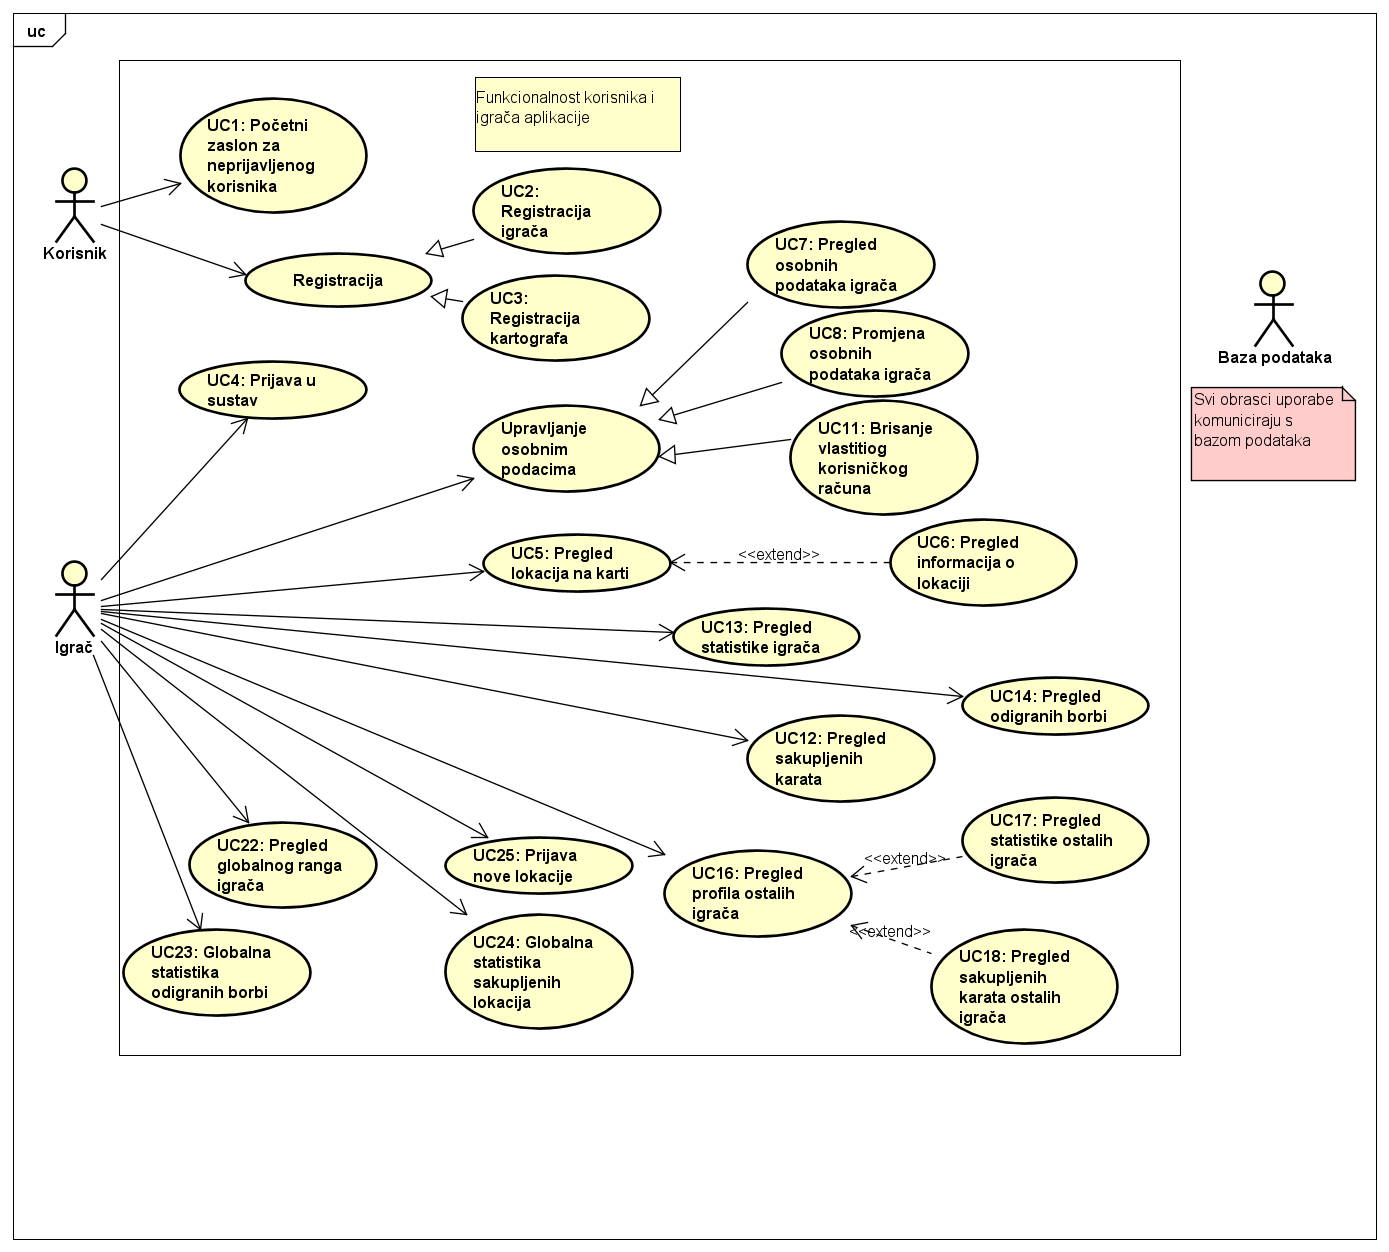
\includegraphics[width=\textwidth, height=16cm]{dijagrami/OU_igrac} 
						\centering
						\caption{Dijagram obrasca uporabe, funkcionalnost korisnika i klijenta}
						\label{}
					\end{figure}
					
					\begin{figure}[H]
						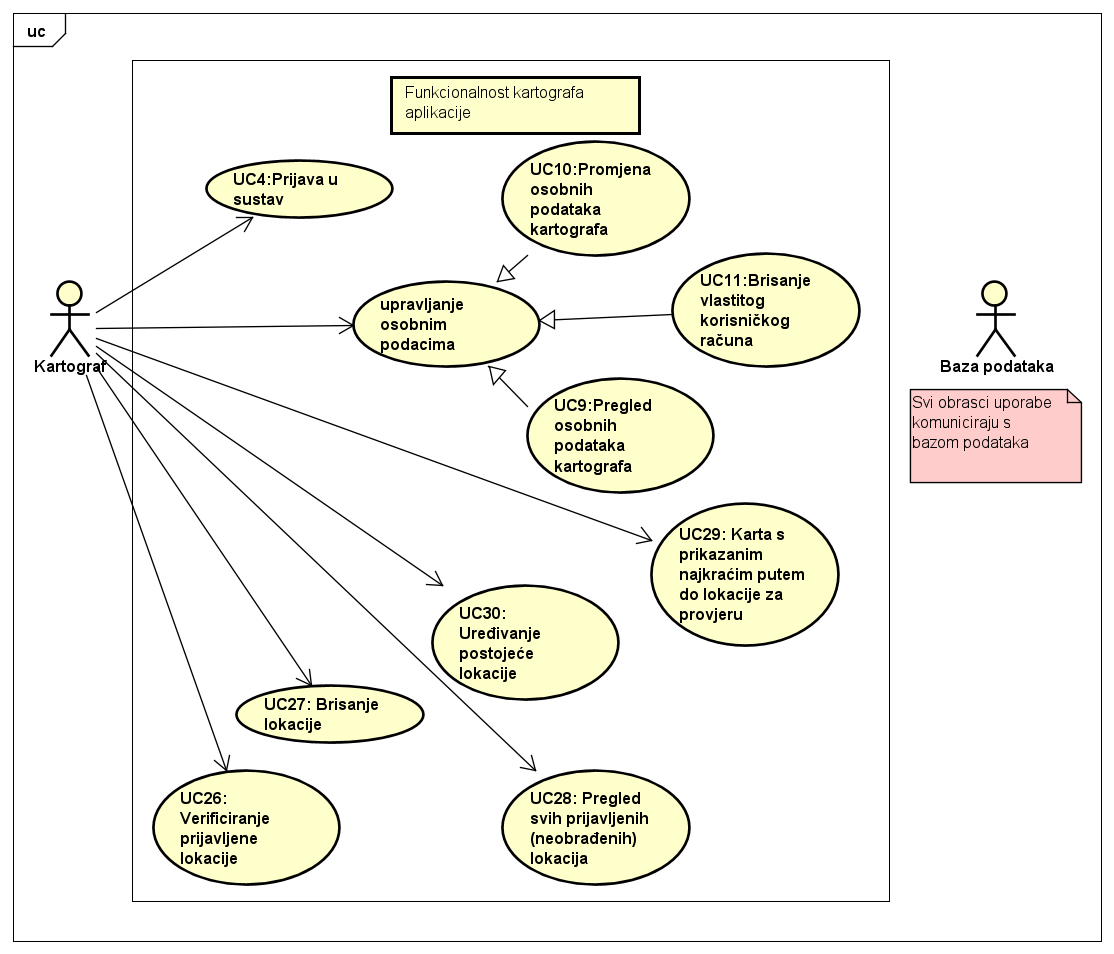
\includegraphics[width=\textwidth, height=14cm]{dijagrami/OU_kartograf}
						\centering
						\caption{Dijagram obrasca uporabe, funkcionalnost kartografa}
						\label{fig:promjene2} %label mora biti drugaciji za svaku sliku
					\end{figure}
				
					\begin{figure}[H]
						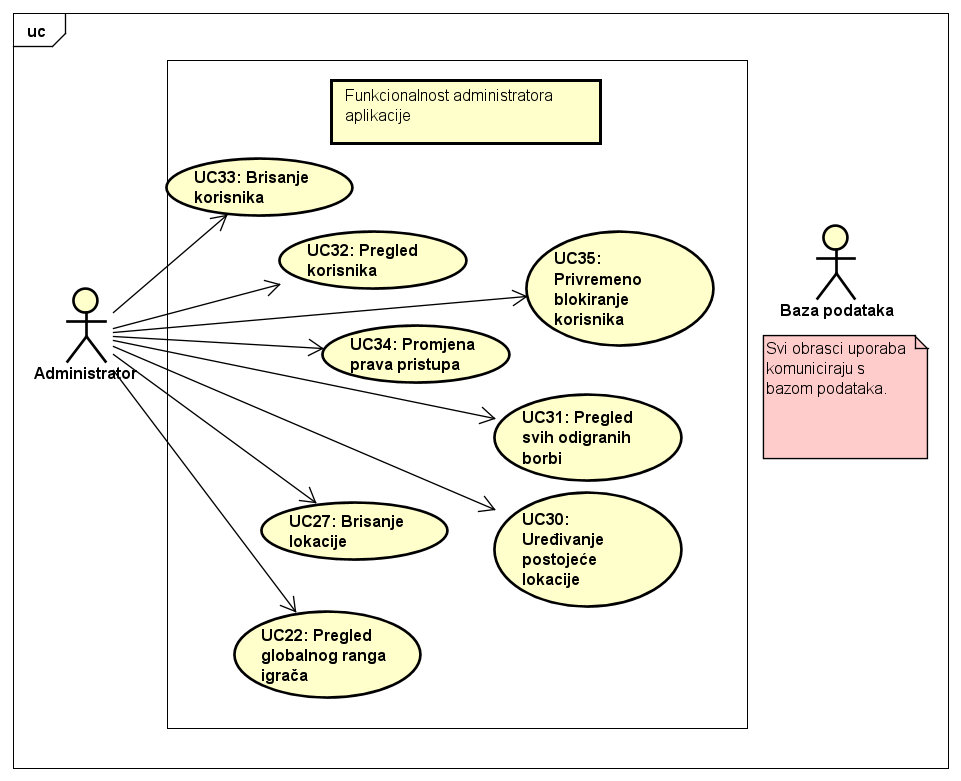
\includegraphics[width=\textwidth, height=12cm]{dijagrami/OU_admin} 
						\centering
						\caption{Dijagram obrasca uporabe, funkcionalnost administratora}
						\label{}
					\end{figure}
					
					
				\eject		
				
			\subsection{Sekvencijski dijagrami}
			
				\textbf{Obrazac uporabe UC5 - Pregled lokacija na karti}\\
					
					{Igrač šalje zahtjev za prikaz karte s lokacijama kako bi mogao odabrati lokaciju koju želi skupiti. Poslužitelj dohvaća lokacije i prikazuje ih. Odabirom lokacije, poslužitelj iz baze podataka dohvaća osnovne podatke o lokaciji i prikazuje ih klijentu. Ako igrač nije skupio karticu, prikazuje mu se opcija da je sakupi. Poslužitelj tu informaciju prosljeđuje bazi koja spremna promjenu.}\\
					
					\begin{figure}[H]
						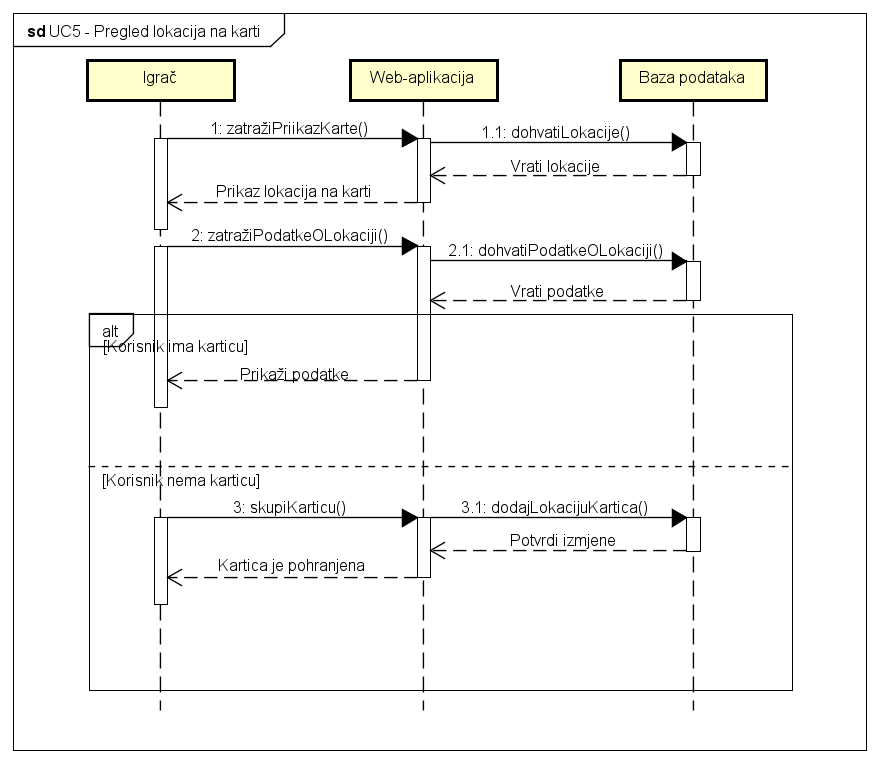
\includegraphics[width=\linewidth, height=14cm]{dijagrami/sd_UC5}
						\centering
						\caption{Sekvencijski dijagram UC5}
						\label{}
					\end{figure}
				\newpage	
				
				\textbf{Obrazac uprabe UC21 - Borba igrača}
					
					{Igrač odabire opciju "Prikaz karata". Poslužitelj dohvaća karte iz baze podataka te ih prikazuje igraču. Igrači biraju 3 karte s kojima će se boriti. Na početku borbe prikazuje se koji igrač igra prvi. Poslužitelj dohvaća globalni rang igrača iz baze podataka te prikazuje igrača koji ima manji globalni rang. Dok ne iskoriste sve 3 izabrane karte, igrači bacaju naizmjenično kartu. Poslužitelj uspoređuje karte te vraća jaču kartu i dodaje bod igraču čija je to karta. Ukoliko su jačine karata jednake, sustav ispiše poruku da je runda izjednačena i nastavlja se borba. Na kraju borbe prikazuje se konačan broj bodova igrača. Igrač koji ima više bodova je pobjednik. Ako igrači imaju jednak broj bodova sustav ispiše poruku da je borba izjednačena.}\\
					
					\begin{figure}[H]
						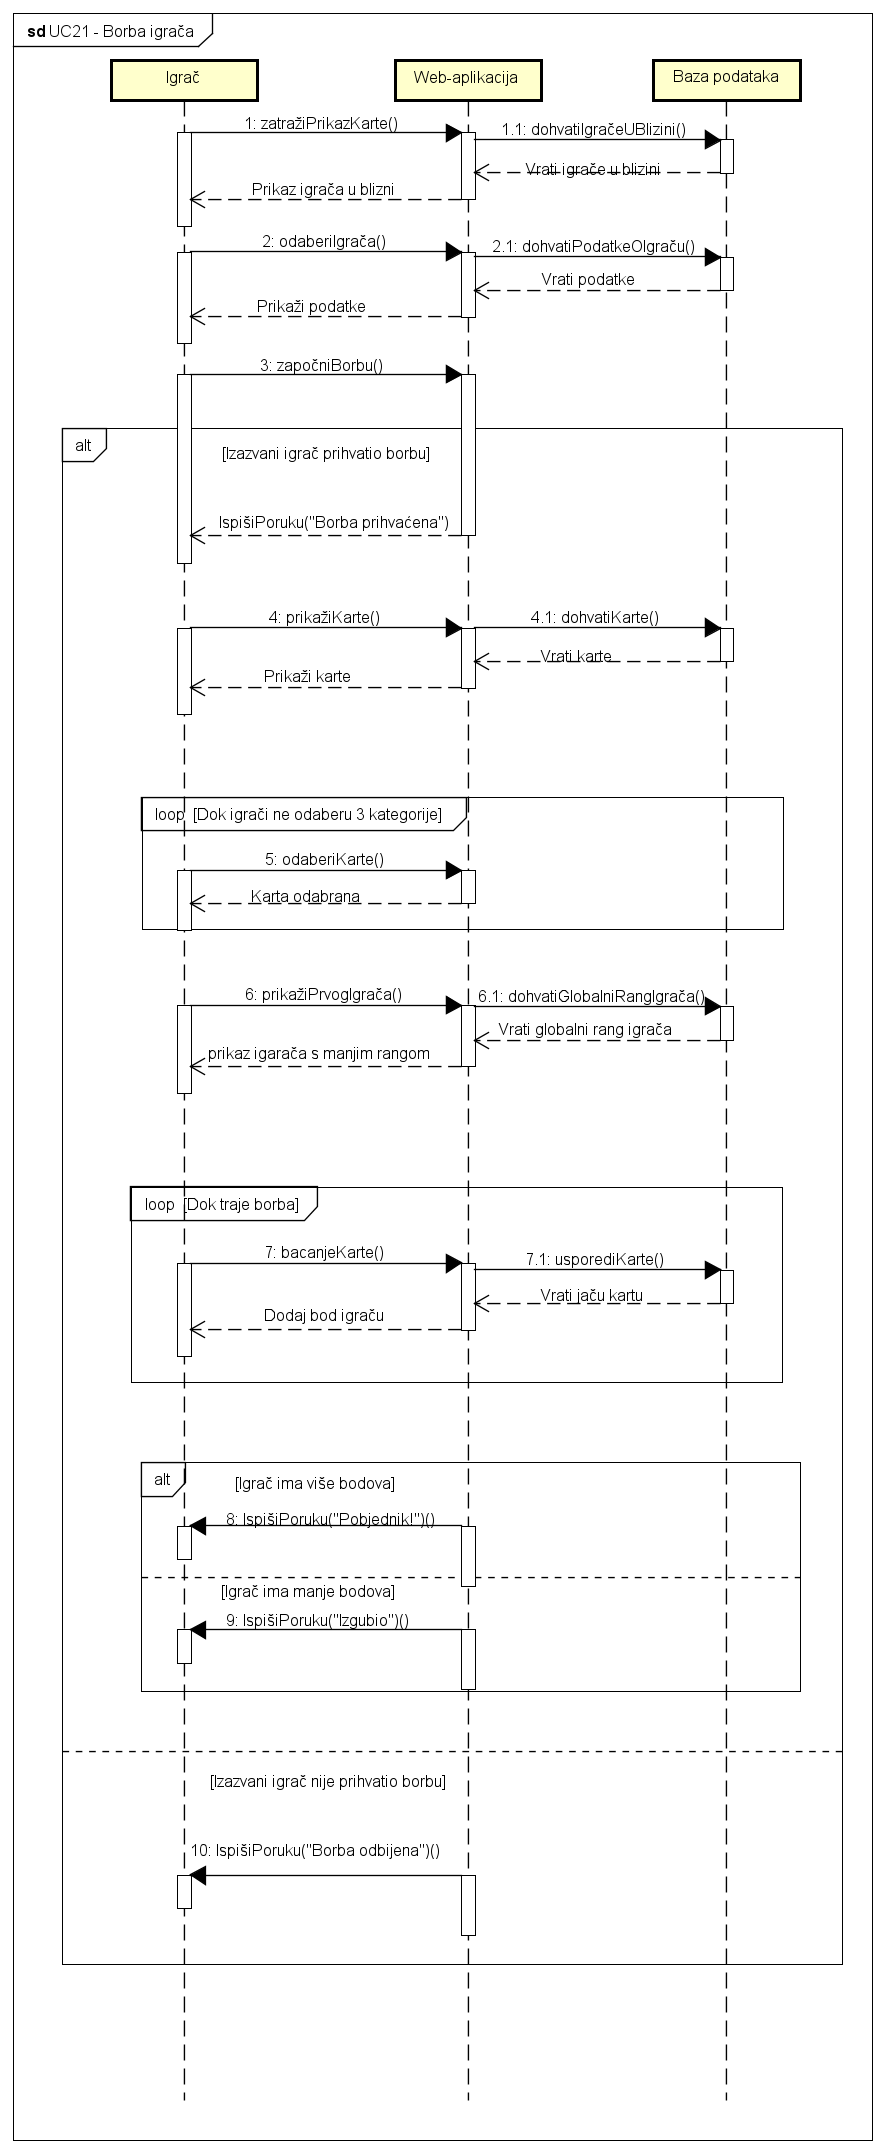
\includegraphics[width=13cm, height=22cm]{dijagrami/sd_UC21}				
						\centering
						\caption{Sekvencijski dijagram UC21}
						\label{}
					\end{figure}
				\newpage
				
				\textbf{Obrazac uporabe UC30 - Uređivanje postojeće lokacije}\\
					
					{Kartograf odabire opciju "Prikaz karte". Poslužitelj dohvaća popis lokacija iz baze podataka te ih prikazuje kartografu na karti. Kartograf odabire lokaciju. Poslužitelj dohvaća podatke o lokaciji iz baze podataka te ih prikazuje kartografu.Kartograf šalje zahtjev za promjenu podataka o lokaciji. Poslužitelj mu daje pristup i kartograf unosi nove podatke o željenoj lokaciji. Poslužitelj izmijeni podatke u bazi podataka koja vraća potvrdu.}\\
					
					\begin{figure}[H]
						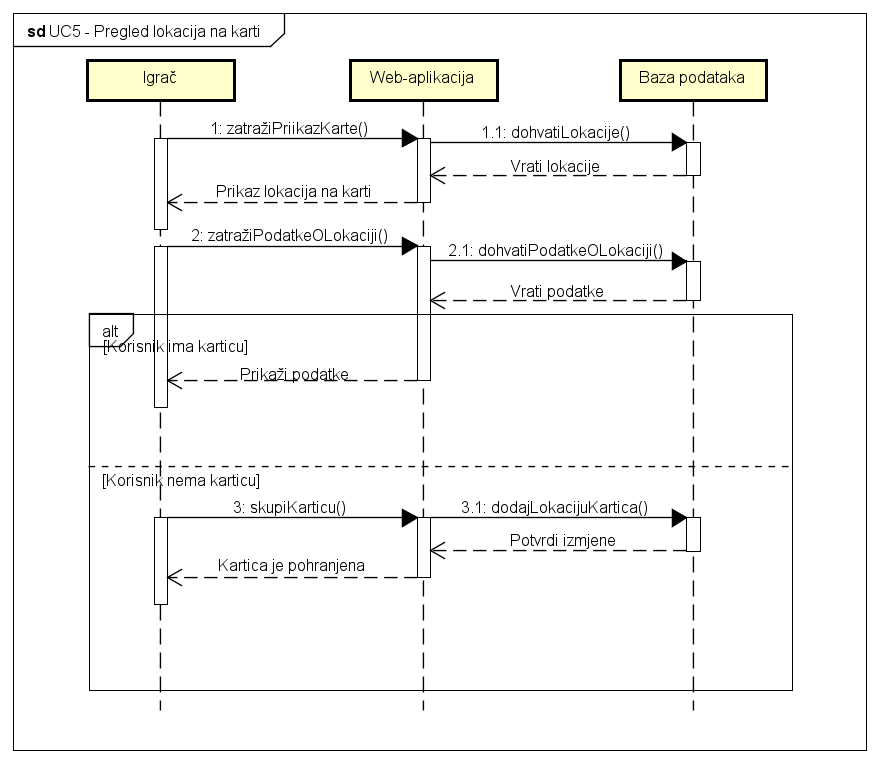
\includegraphics[width=\linewidth, height=14cm]{dijagrami/sd_UC30}				
						\centering
						\caption{Sekvencijski dijagram UC30}
						\label{}
					\end{figure}
					
				
				\eject
	
		\section{Ostali zahtjevi}
		
			\begin{packed_item}
				\item Sustav treba omogućiti rad više korisnika u stvarnom vremenu 
				\item Korisničko sučelje i sustav moraju podržavati hrvatsku abecedu (dijakritičke znakove) pri unosu tekstualnog sadržaja
				\item Izvršavanje dijela programa u kojem se pristupa bazi podataka ne smije trajati duže od nekoliko sekundi
				\item Sustav treba biti implementiran kao web aplikacija koristeći objektno-orijentirane jezike
				\item Neispravno korištenje korisničkog sučelja ne smije narušiti funkcionalnost i rad sustava
				\item Sustav treba biti jednostavan za korištenje, korisnici se moraju znati koristiti sučeljem bez opširnih uputa
				\item Nadogradnja sustava ne smije narušavati postojeće funkcionalnosti sustava
				\item Veza s bazom podataka mora biti kvalitetno zaštićena, brza i otporna na vanjske greške
				\item Pristup sustavu mora biti omogućen iz javne mreže pomoću HTTPS.
			\end{packed_item}
			 
			 
			 
	
	\chapter{Arhitektura i dizajn sustava}
		
		\textbf{\textit{dio 1. revizije}}\\

		\textit{ Potrebno je opisati stil arhitekture te identificirati: podsustave, preslikavanje na radnu platformu, spremišta podataka, mrežne protokole, globalni upravljački tok i sklopovsko-programske zahtjeve. Po točkama razraditi i popratiti odgovarajućim skicama:}
	\begin{itemize}
		\item 	\textit{izbor arhitekture temeljem principa oblikovanja pokazanih na predavanjima (objasniti zašto ste baš odabrali takvu arhitekturu)}
		\item 	\textit{organizaciju sustava s najviše razine apstrakcije (npr. klijent-poslužitelj, baza podataka, datotečni sustav, grafičko sučelje)}
		\item 	\textit{organizaciju aplikacije (npr. slojevi frontend i backend, MVC arhitektura) }		
	\end{itemize}

	
		

		

				
		\section{Baza podataka}
			
			\textbf{\textit{dio 1. revizije}}\\
			
		\textit{Potrebno je opisati koju vrstu i implementaciju baze podataka ste odabrali, glavne komponente od kojih se sastoji i slično.}
		
			\subsection{Opis tablica}
			

				{\textbf{Location}	Ovaj entitet sadržava sve važne informacije o lokacijama na kojima igrač može sakupiti karte. Sadrži atribute: ID lokacije, naziv lokacije, fotografiju lokacije i ID kategorije. Ovaj entitet u vezi je \textit{Many-to-One} s Category preko ID kategorije.}
				
				\begin{longtabu} to \textwidth {|X[6, l]|X[6, l]|X[20, l]|}
					
					\hline \multicolumn{3}{|c|}{\textbf{location}}	 \\[3pt] \hline
					\endfirsthead
					
					\hline \multicolumn{3}{|c|}{\textbf{location}}	 \\[3pt] \hline
					\endhead
					
					\hline 
					\endlastfoot
					
					\cellcolor{LightGreen}location\_id & INT	&   jedinstveni brojčani identifikator lokacije	\\ \hline
					location\_name	& VARCHAR &  naziv lokacije 	\\ \hline 
					location\_photo & UUID &  fotografija lokacije \\ \hline 
					\cellcolor{LightBlue} category\_id	& INT &   jedinstveni brojčani identifikator kategorije	\\ \hline 
					
					
				\end{longtabu}
			
				{\textbf{Category}	Ovaj entitet sadržava sve važne informacije o kategorijama koje lokacije mogu biti. Sadrži atribute: ID kategorije, naziv kategorije i broj bodova koje kategorija nosi. Ovaj entitet u vezi je \textit{One-to-Many} s Location preko ID kategorije.}
				
				\begin{longtabu} to \textwidth {|X[6, l]|X[6, l]|X[20, l]|}
					
					\hline \multicolumn{3}{|c|}{\textbf{category}}	 \\[3pt] \hline
					\endfirsthead
					
					\hline \multicolumn{3}{|c|}{\textbf{category}}	 \\[3pt] \hline
					\endhead
					
					\hline 
					\endlastfoot
					
					\cellcolor{LightGreen}category\_id & INT	&   jedinstveni brojčani identifikator kategorije	\\ \hline
					category\_name	& VARCHAR &  naziv kategorije 	\\ \hline 
					category\_points & INT &  bodovna vrijednost kategorije \\ \hline  
					
					
				\end{longtabu}
			
				{\textbf{Card}	Ovaj entitet sadržava sve važne informacije o kartama koje igrači mogu posjedovati. Sadrži atribute: ID karte, broj bodova koje karte i ID lokacije. Ovaj entitet u vezi je \textit{Many-to-One} s Location preko ID lokacije te \textit{Many-to-One} s Deck preko ID karte.}

				\begin{longtabu} to \textwidth {|X[6, l]|X[6, l]|X[20, l]|}
					
					\hline \multicolumn{3}{|c|}{\textbf{card}}	 \\[3pt] \hline
					\endfirsthead
					
					\hline \multicolumn{3}{|c|}{\textbf{card}}	 \\[3pt] \hline
					\endhead
					
					\hline 
					\endlastfoot
					
					\cellcolor{LightGreen}card\_id & INT	&   jedinstveni brojčani identifikator karte	\\ \hline 
					card\_points & INT &  bodovna vrijednost karte \\ \hline 
					\cellcolor{LightBlue} location\_id	& INT &   jedinstveni brojčani identifikator lokacije	\\ \hline 
					
					
				\end{longtabu}
			
				{\textbf{Deck}	Ovaj entitet sadržava sve važne informacije o špilu koje igrač posjeduje. Sadrži atribute: korisničko ime i ID karte. Ovaj entitet u vezi je \textit{One-to-One} s Player preko korisničkog imena te \textit{One-to-Many} s Deck preko ID karte.}
				
				\begin{longtabu} to \textwidth {|X[6, l]|X[6, l]|X[20, l]|}
					
					\hline \multicolumn{3}{|c|}{\textbf{deck}}	 \\[3pt] \hline
					\endfirsthead
					
					\hline \multicolumn{3}{|c|}{\textbf{deck}}	 \\[3pt] \hline
					\endhead
					
					\hline 
					\endlastfoot
					
					\cellcolor{LightBlue}username & VARCHAR	&   korisničko ime igrača	\\ \hline
					\cellcolor{LightBlue} card\_id	& INT &   jedinstveni brojčani identifikator karte	\\ \hline 
					
					
				\end{longtabu}
			
			
			\subsection{Dijagram baze podataka}
				\begin{figure}[H]
					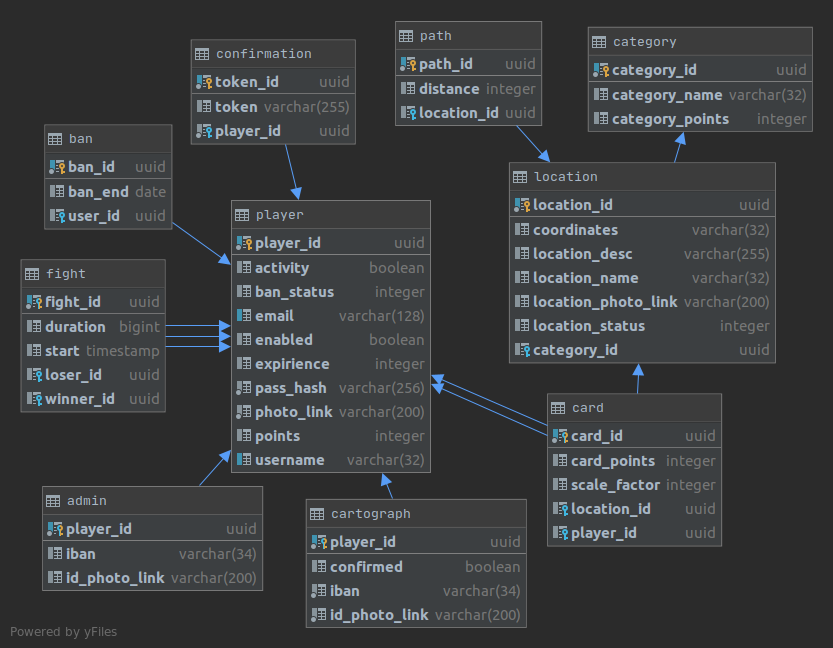
\includegraphics[width=\linewidth, height=14cm]{dijagrami/geofighterdb_diagram}				
					\centering
					\caption{E-R dijagram baze podataka}
					\label{}
				\end{figure}
			
			\eject
			
			
		\section{Dijagram razreda}
		
			\textit{Potrebno je priložiti dijagram razreda s pripadajućim opisom. Zbog preglednosti je moguće dijagram razlomiti na više njih, ali moraju biti grupirani prema sličnim razinama apstrakcije i srodnim funkcionalnostima.}\\
			
			\textbf{\textit{dio 1. revizije}}\\
			
			\textit{Prilikom prve predaje projekta, potrebno je priložiti potpuno razrađen dijagram razreda vezan uz \textbf{generičku funkcionalnost} sustava. Ostale funkcionalnosti trebaju biti idejno razrađene u dijagramu sa sljedećim komponentama: nazivi razreda, nazivi metoda i vrste pristupa metodama (npr. javni, zaštićeni), nazivi atributa razreda, veze i odnosi između razreda.}\\
			
			\textbf{\textit{dio 2. revizije}}\\			
			
			\textit{Prilikom druge predaje projekta dijagram razreda i opisi moraju odgovarati stvarnom stanju implementacije}
			
			
			
			\eject
		
%		\section{Dijagram stanja}
%			
%			
%			\textbf{\textit{dio 2. revizije}}\\
%			
%			\textit{Potrebno je priložiti dijagram stanja i opisati ga. Dovoljan je jedan dijagram stanja koji prikazuje \textbf{značajan dio funkcionalnosti} sustava. Na primjer, stanja korisničkog sučelja i tijek korištenja neke ključne funkcionalnosti jesu značajan dio sustava, a registracija i prijava nisu. }
%			
%			
%			\eject 
%		
%		\section{Dijagram aktivnosti}
%			
%			\textbf{\textit{dio 2. revizije}}\\
%			
%			 \textit{Potrebno je priložiti dijagram aktivnosti s pripadajućim opisom. Dijagram aktivnosti treba prikazivati značajan dio sustava.}
%			
%			\eject
%		\section{Dijagram komponenti}
%		
%			\textbf{\textit{dio 2. revizije}}\\
%		
%			 \textit{Potrebno je priložiti dijagram komponenti s pripadajućim opisom. Dijagram komponenti treba prikazivati strukturu cijele aplikacije.}
	\chapter{Implementacija i korisničko sučelje}
		
		
		\section{Korištene tehnologije i alati}
		
			\textbf{\textit{dio 2. revizije}}
			
			 \textit{Detaljno navesti sve tehnologije i alate koji su primijenjeni pri izradi dokumentacije i aplikacije. Ukratko ih opisati, te navesti njihovo značenje i mjesto primjene. Za svaki navedeni alat i tehnologiju je potrebno \textbf{navesti internet poveznicu} gdje se mogu preuzeti ili više saznati o njima}.
			
			
			\eject 
		
	
		\section{Ispitivanje programskog rješenja}
			
			\textbf{\textit{dio 2. revizije}}\\
			
			 \textit{U ovom poglavlju je potrebno opisati provedbu ispitivanja implementiranih funkcionalnosti na razini komponenti i na razini cijelog sustava s prikazom odabranih ispitnih slučajeva. Studenti trebaju ispitati temeljnu funkcionalnost i rubne uvjete.}
	
			
			\subsection{Ispitivanje komponenti}
			\textit{Potrebno je provesti ispitivanje jedinica (engl. unit testing) nad razredima koji implementiraju temeljne funkcionalnosti. Razraditi \textbf{minimalno 6 ispitnih slučajeva} u kojima će se ispitati redovni slučajevi, rubni uvjeti te izazivanje pogreške (engl. exception throwing). Poželjno je stvoriti i ispitni slučaj koji koristi funkcionalnosti koje nisu implementirane. Potrebno je priložiti izvorni kôd svih ispitnih slučajeva te prikaz rezultata izvođenja ispita u razvojnom okruženju (prolaz/pad ispita). }
			
			
			
			\subsection{Ispitivanje sustava}
			
			 \textit{Potrebno je provesti i opisati ispitivanje sustava koristeći radni okvir Selenium\footnote{\url{https://www.seleniumhq.org/}}. Razraditi \textbf{minimalno 4 ispitna slučaja} u kojima će se ispitati redovni slučajevi, rubni uvjeti te poziv funkcionalnosti koja nije implementirana/izaziva pogrešku kako bi se vidjelo na koji način sustav reagira kada nešto nije u potpunosti ostvareno. Ispitni slučaj se treba sastojati od ulaza (npr. korisničko ime i lozinka), očekivanog izlaza ili rezultata, koraka ispitivanja i dobivenog izlaza ili rezultata.\\ }
			 
			 \textit{Izradu ispitnih slučajeva pomoću radnog okvira Selenium moguće je provesti pomoću jednog od sljedeća dva alata:}
			 \begin{itemize}
			 	\item \textit{dodatak za preglednik \textbf{Selenium IDE} - snimanje korisnikovih akcija radi automatskog ponavljanja ispita	}
			 	\item \textit{\textbf{Selenium WebDriver} - podrška za pisanje ispita u jezicima Java, C\#, PHP koristeći posebno programsko sučelje.}
			 \end{itemize}
		 	\textit{Detalji o korištenju alata Selenium bit će prikazani na posebnom predavanju tijekom semestra.}
			
			\eject 
		
		
		\section{Dijagram razmještaja}
			
			%\textbf{\textit{dio 2. revizije}}
			
			 %\textit{Potrebno je umetnuti \textbf{specifikacijski} dijagram razmještaja i opisati ga. Moguće je umjesto specifikacijskog dijagrama razmještaja umetnuti dijagram razmještaja instanci, pod uvjetom da taj dijagram bolje opisuje neki važniji dio sustava.}
			
			{Dijagrami razmještaja (engl. deployment diagrams) opisuju topologiju skopovlja i programsku potporu koja se koristi u implementaciji sustava u njegovom radnom i produkcijskom okruženju. Dijagram razmještaja prikazuje razvijene aplikacije. Na poslužiteljskom računalu nalaze se web poslužitelj, poslužitelj baze podataka te poslužitelji Cloudinary i OSRM. Kako bi pristupili web aplikaciji, klijenti koriste web preglednik. Razmjena podataka između korisnika (igrač, kartograf, admin) i poslužitelja odvija se korištenjem HTTP protokola.}
			\begin{figure}[H]
				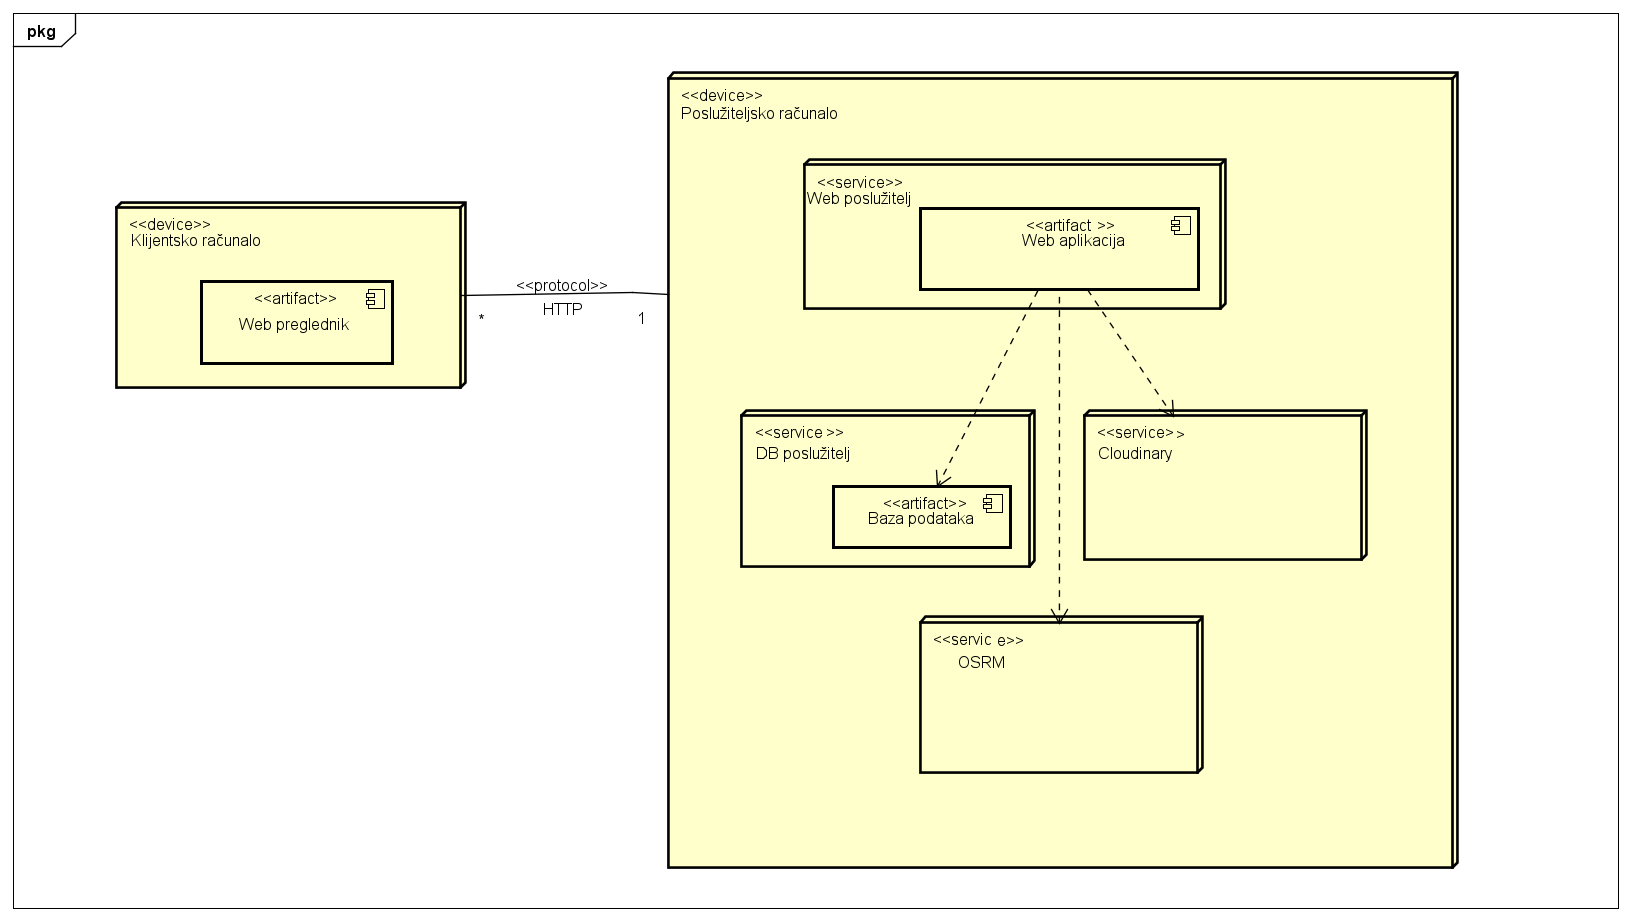
\includegraphics[width=\textwidth]{dijagrami/dijagram_razmjestaja} 
				\centering
				\caption{Dijagram razmještaja}
				\label{}
			\end{figure}
			\eject 
		
		\section{Upute za puštanje u pogon}
		
			\textbf{\textit{dio 2. revizije}}\\
		
			 \textit{U ovom poglavlju potrebno je dati upute za puštanje u pogon (engl. deployment) ostvarene aplikacije. Na primjer, za web aplikacije, opisati postupak kojim se od izvornog kôda dolazi do potpuno postavljene baze podataka i poslužitelja koji odgovara na upite korisnika. Za mobilnu aplikaciju, postupak kojim se aplikacija izgradi, te postavi na neku od trgovina. Za stolnu (engl. desktop) aplikaciju, postupak kojim se aplikacija instalira na računalo. Ukoliko mobilne i stolne aplikacije komuniciraju s poslužiteljem i/ili bazom podataka, opisati i postupak njihovog postavljanja. Pri izradi uputa preporučuje se \textbf{naglasiti korake instalacije uporabom natuknica} te koristiti što je više moguće \textbf{slike ekrana} (engl. screenshots) kako bi upute bile jasne i jednostavne za slijediti.}
			
			
			 \textit{Dovršenu aplikaciju potrebno je pokrenuti na javno dostupnom poslužitelju. Studentima se preporuča korištenje neke od sljedećih besplatnih usluga: \href{https://aws.amazon.com/}{Amazon AWS}, \href{https://azure.microsoft.com/en-us/}{Microsoft Azure} ili \href{https://www.heroku.com/}{Heroku}. Mobilne aplikacije trebaju biti objavljene na F-Droid, Google Play ili Amazon App trgovini.}
			
			
			\eject 
	\chapter{Zaključak i budući rad}
		
		{Zadatak naše grupe bio je razvoj igre \textit{GeoFighter} u kojoj se igrači međusobno bore kartama. Igrači karte skupljaju na različitim stvarnim lokacijama, a cilj razvoja igre je popunjavanje manjkave baze podataka stvarnih lokacija. Nakon 15 tjedana timskog rada u razvijanju igre, uspješno smo ostvarili zadani cilj. Provedba projekta izvodila se kroz dvije faze.} 
		
		{Prva faza projekta uključivala je okupljanje tima za razvoj igrice, dodjele projektnih zadataka, formiranje podtimova za rad na \textit{frontendu} i \textit{backendu} te dokumentiranje zahtjeva igre. Kvalitetnim dokumentiranjem tijekom prve faze projekta uvelike smo olakšali daljnju implementaciju i rad na samoj igri te osmišljavanju sustava. Izrađeni obrasci i dijagrami (obrasci uporabe, sekvencijski dijagrami, model bazepodataka, dijagram razreda) pomogli su timovima za razvoj \textit{frontenda} i \textit{backenda} koje smo definirali u ranijem dijelu prve faze te su uštedili mnogo vremena tijekom druge faze projekta kada su članovi tima nailazili na nedoumice oko implementacije rješenja.}
			
		{Druga faza projekta uglavnom se temeljila na samostalnom radu članova te na stjecanju novih znanja u slučaju manjka iskustva pri korištenju potrebnih odabranih alata i programskih jezika za izradu implementacijskih rješenja. Također, u drugoj fazi bilo je potrebno dovršiti i dokumentirati ostale UML dijagrame i napisati ostatak dokumentacije projekta. Temeljito dokumentirano željeno ponašanje sustava te dobro izrađeni obrasci i dijagrami tijekom prve faze projekta omogućili su nam da izbjegnemo potencijalne pogreške tijekom razvoja igre koje bi bile vremenski skupe u daljnjoj izradi projekta.}
		
		{Moguće proširenje postojeće inačice sustava je izrada mobilne aplikacije čime bi korisničko iskustvo bilo bogatije i bolje nego ono ostvareno web aplikacijom. Moguće su nadogradnje u obliku organiziranih turnira i dodavanju mogućnosti za proširenje udaljenosti za borbu kao i dodavanje različitih tipova borbi.}
		
		{Sudjelovanje na ovom projektu naučilo nas je koliko znači dobra komunikacija među članovima tima, koliko je nužno međusobno poštivanje i razumijevanje prema kolegama u timu te važnost dobre vremenske organiziranosti i koordiniranosti među članovima. Naposljetku, iako zadovoljni postignutim rezultatima i stečenim iskustvima tijekom rada na projektnom zadatku, svjesni smo potencijalnih nadogradnji kao i onih dijelova koje smo mogli bolje implementirati. Bez obzira na to, puno smo naučili.}\textsc{}
		
		\eject 
	\chapter*{Popis literature}
		\addcontentsline{toc}{chapter}{Popis literature}
		
		
		\begin{enumerate}
			
			
			\item  Programsko inženjerstvo, FER ZEMRIS, \url{http://www.fer.hr/predmet/proinz}
			
			\item  Astah Community, \url{http://astah.net/editions/uml-new}
			
			\item Spring Boot, \url{https://spring.io/}
			
			\item React, \url{https://reactjs.org}
			
			\item Java and Databases, \url{https://www.marcobehler.com/guides/java-databases}
			
			\item EDRPlus, \url{https://erdplus.com}
			
			\item DataGrip, \url{https://www.jetbrains.com/datagrip/}
			
			\item Spring Data JPA, \url{https://spring.io/projects/spring-data-jpa}
			
			\item Eclipse, \url{https://www.eclipse.org}
			
			\item Visual Studio Code, \url{https://code.visualstudio.com}
			
			%\item  I. Sommerville, "Software engineering", 8th ed, Addison Wesley, 2007.
			
			%\item  T.C.Lethbridge, R.Langaniere, "Object-Oriented Software Engineering", 2nd ed. McGraw-Hill, 2005.
			
			%\item  I. Marsic, Software engineering book``, Department of Electrical and Computer Engineering, Rutgers University, \url{http://www.ece.rutgers.edu/~marsic/books/SE}
			
			%\item  The Unified Modeling Language, \url{https://www.uml-diagrams.org/}
			
		\end{enumerate}
		
		 
	
	
	\begingroup
	\renewcommand*\listfigurename{Indeks slika i dijagrama}
	%\renewcommand*\listtablename{Indeks tablica}
	%\let\clearpage\relax
	\listoffigures
	%\vspace{10mm}
	%\listoftables
	\endgroup
	\addcontentsline{toc}{chapter}{Indeks slika i dijagrama}


	
	\eject 
		
	\chapter*{Dodatak: Prikaz aktivnosti grupe}
		\addcontentsline{toc}{chapter}{Dodatak: Prikaz aktivnosti grupe}
		
		\section*{Dnevnik sastajanja}
		
		\begin{packed_enum}
			\item  sastanak
			
			\item[] \begin{packed_item}
				\item Datum: 6. listopada 2020.
				\item Prisustvovali: M.Frandolić, L.Bašić, L.Brečić, P.Kopić, I.Krivačić, N.Petrović
				\item Teme sastanka:
				\begin{packed_item}
					\item sastanak s asistentom i demonstratorom
					\item analiza zadatka
					\item raščišćavanje osnovnih dilema funkcionalnosti
					\item okviran odabir alata i tehnologija
				\end{packed_item}
			\end{packed_item}
		
			\item sastanak
			\item[] \begin{packed_item}
				\item Datum: 10. listopada 2020.
				\item Prisustvovali: M.Frandolić, L.Bašić, L.Brečić, P.Kopić, I.Krivačić, N.Petrović
				\item Teme sastanka:
				\begin{packed_item}
					\item konačan odabir alata i tehnologija
					\item definiranje opisa projektnog zadatka
					\item definiranje funkcionalnih zahtjeva
					\item podjela opisa obrazaca uporabe
				\end{packed_item}
			\end{packed_item}
			
			\item  sastanak
			\item[] \begin{packed_item}
				\item Datum: 19. listopada 2020.
				\item Prisustvovali: M.Frandolić, I.Krivačić
				\item Teme sastanka:
				\begin{packed_item}
					\item kratko predavanje demosa na temu CI/CD
				\end{packed_item}
			\end{packed_item}
			\newpage
			\item sastanak
			\item[] \begin{packed_item}
				\item Datum: 21. listopada 2020.
				\item Prisustvovali: M.Frandolić, L.Bašić, L.Brečić, P.Kopić, I.Krivačić, N.Petrović
				\item Teme sastanka:
				\begin{packed_item}
					\item sastanak s asistentom - dikusija o postojećim sličnim aplikacijama, potencijalnoj koristi projekta, moguće nadogradnje projektnog zadatka te rješavanje nejasnoća oko obrazaca uporabe
					\item podjela zadatka(dijagrami obrazaca uporabe, sekvencijski dijagrami, baza podataka)
				\end{packed_item}
			\end{packed_item}
		
			\item sastanak
			\item[] \begin{packed_item}
				\item Datum: 30. listopada 2020.
				\item Prisustvovali: M.Frandolić, I.Krivačić
				\item Teme sastanka:
				\begin{packed_item}
					\item sastanak s asistentom - diskusija o ispravnosti i nadopuni dijagarma obrazaca i sekvencijskih dijagrama
				\end{packed_item}
			\end{packed_item}
			
			\item sastanak
			\item[] \begin{packed_item}
				\item Datum: 31. listopada 2020.
				\item Prisustvovali: M.Frandolić, L.Bašić, L.Brečić, P.Kopić, I.Krivačić, N.Petrović
				\item Teme sastanka:
				\begin{packed_item}
					\item podjela zadataka za frontend (početna stranica i mogućnost registracije), backend (funkcionalnost za registraciju, povezivanje s frontendom)
					\item podjela posla za bazu podataka
				\end{packed_item}
			\end{packed_item}
		
			\item sastanak
			\item[] \begin{packed_item}
				\item Datum: 6. studenoga 2020.
				\item Prisustvovali: M.Frandolić, L.Bašić, L.Brečić, P.Kopić, N.Petrović
				\item Teme sastanka:
				\begin{packed_item}
					\item sastanak s asistentom 
					\item rasprava o bazi podataka
				\end{packed_item}
			\end{packed_item}
			\newpage
			\item sastanak
			\item[] \begin{packed_item}
				\item Datum: 7. studenoga 2020.
				\item Prisustvovali: M.Frandolić, L.Bašić, L.Brečić, P.Kopić, I.Krivačić, N.Petrović
				\item Teme sastanka:
				\begin{packed_item}
					\item rasprava o implementaciji baze podataka
					\item raspravljanje o napravljenom frontendu i backendu
					\item daljnja podjela posla za frontend(prikaz početnih stranica za igrača, admina i kartografa)
				\end{packed_item}
			\end{packed_item}
			
			\item sastanak
			\item[] \begin{packed_item}
				\item Datum: 11. studenoga 2020.
				\item Prisustvovali: M.Frandolić, L.Bašić, L.Brečić, P.Kopić, I.Krivačić, N.Petrović
				\item Teme sastanka:
				\begin{packed_item}
					\item sastanak s asistentom i demonstratorom - demonstracija dosadašnjeg rada
					\item podjela preostale dokumentacije
				\end{packed_item}
			\end{packed_item}
			
			%
			
		\end{packed_enum}
		
		\eject
		\section*{Tablica aktivnosti}
			
			
			\begin{longtabu} to \textwidth {|X[7, l]|X[1, c]|X[1, c]|X[1, c]|X[1, c]|X[1, c]|X[1, c]|X[1, c]|}
								
				\cline{2-8} \multicolumn{1}{c|}{\textbf{}} &     \multicolumn{1}{c|}{\rotatebox{90}{\textbf{Matija Frandolić }}} & \multicolumn{1}{c|}{\rotatebox{90}{\textbf{Lukas Bašić }}} &	\multicolumn{1}{c|}{\rotatebox{90}{\textbf{Luka Brečić }}} &	\multicolumn{1}{c|}{\rotatebox{90}{\textbf{Palma Kopić }}} &
				\multicolumn{1}{c|}{\rotatebox{90}{\textbf{Ivana Krivačić }}} &
				\multicolumn{1}{c|}{\rotatebox{90}{\textbf{Nikola Petrović }}} &	\multicolumn{1}{c|}{\rotatebox{90}{\textbf{Ozren Skerlev  }}} \\ \hline 
				\endfirsthead
				
			
				\cline{2-8} \multicolumn{1}{c|}{\textbf{}} &     \multicolumn{1}{c|}{\rotatebox{90}{\textbf{Matija Frandolić}}} & \multicolumn{1}{c|}{\rotatebox{90}{\textbf{Lukas Bašić }}} &	\multicolumn{1}{c|}{\rotatebox{90}{\textbf{Luka Brečić }}} &
				\multicolumn{1}{c|}{\rotatebox{90}{\textbf{Palma Kopić }}} &	\multicolumn{1}{c|}{\rotatebox{90}{\textbf{Ivana Krivačić }}} &
				\multicolumn{1}{c|}{\rotatebox{90}{\textbf{Nikola Petrović }}} &	\multicolumn{1}{c|}{\rotatebox{90}{\textbf{Ozren Skerlev }}} \\ \hline 
				\endhead
				
				
				\endfoot
							
				 
				\endlastfoot
				
				Upravljanje projektom 		&  &  &  &  &  &  & \\ \hline
				Opis projektnog zadatka 	&  &  &  & 9 &  &  & \\ \hline
				
				Funkcionalni zahtjevi       &  &  &  &  &  &  &  \\ \hline
				Opis pojedinih obrazaca 	&  &  &  &  & 6 &  &  \\ \hline
				Dijagram obrazaca 			&  &  &  &  & 4 &  &  \\ \hline
				Sekvencijski dijagrami 		&  &  &  &  & 4 &  &  \\ \hline
				Opis ostalih zahtjeva 		&  &  &  &  & 1 &  &  \\ \hline

				Arhitektura i dizajn sustava	 &  &  &  &  & 2 &  &  \\ \hline
				Baza podataka				&  &  &  &  &  &  &   \\ \hline
				Dijagram razreda 			&  &  &  &  &  &  &   \\ \hline
				Dijagram stanja				&  &  &  &  &  &  &  \\ \hline
				Dijagram aktivnosti 		&  &  &  &  &  &  &  \\ \hline
				Dijagram komponenti			&  &  &  &  &  &  &  \\ \hline
				Korištene tehnologije i alati 		&  &  &  &  &  &  &  \\ \hline
				Ispitivanje programskog rješenja 	&  &  &  &  &  &  &  \\ \hline
				Dijagram razmještaja			&  &  &  &  &  &  &  \\ \hline
				Upute za puštanje u pogon 		&  &  &  &  &  &  &  \\ \hline 
				Dnevnik sastajanja 			&  &  &  &  & 2 &  &  \\ \hline
				Zaključak i budući rad 		&  &  &  &  &  &  &  \\  \hline
				Popis literature 			&  &  &  &  &  &  &  \\  \hline
				&  &  &  &  &  &  &  \\ \hline \hline
				\textit{izrada početne stranice} 				&  &  &  &  &  &  &  \\ \hline 
				\textit{izrada baze podataka} 		 			&  &  &  &  &  &  & \\ \hline 
				\textit{spajanje s bazom podataka} 							&  &  &  &  &  &  &  \\ \hline
				\textit{back end} 							&  &  &  &  &  &  &  \\  \hline
				 							&  &  &  &  &  &  &\\  \hline
				
				
			\end{longtabu}
					
					
		\eject
%		\section*{Dijagrami pregleda promjena}
%		
%		\textbf{\textit{dio 2. revizije}}\\
%		
%		\textit{Prenijeti dijagram pregleda promjena nad datotekama projekta. Potrebno je na kraju projekta generirane grafove s gitlaba prenijeti u ovo poglavlje dokumentacije. Dijagrami za vlastiti projekt se mogu preuzeti s gitlab.com stranice, u izborniku Repository, pritiskom na stavku Contributors.}
		
	


\end{document} %naredbe i tekst nakon ove naredbe ne ulaze u izgrađen dokument 


